% First page for bachelor thesis at LIACS: bachelorpage.tex
% Invullen titel, naam+ nummer, datum en begeleiders.
% Version 1.053 Juni 2014 (studentnummer weggehaald)
% Version 1.000 November 2013 (aanpassing oude versie WAK met begeleiders)

% Usage: 
%   latex bachelorpage.tex
%   dvips -Ppdf bachelorpage.dvi
%   ps2pdf bachelorpage.ps
% Needed: file ullogo.eps for the university logo
%
%  concatenate bachelorpage.pdf with yourthesis.pdf to yourfinalthesis.pdf by means of
%  gs -q -sPAPERSIZE=a4 -dNOPAUSE -dBATCH -sDEVICE=pdfwrite -sOutputFile=yourfinalthesis.pdf bachelorpage.pdf yourthesis.pdf

% LIACS thesis skeleton (outline only) — updated project scope
\documentclass[12pt]{article}
\usepackage[a4paper,margin=1in]{geometry}
\usepackage{hyperref}
\usepackage{graphicx}
\usepackage{listings}
\usepackage{enumitem}
\usepackage{amsmath}
\usepackage{booktabs}
\usepackage{url}
\usepackage{titlesec}
\usepackage[most]{tcolorbox}
\usepackage{ebgaramond}
\usepackage{graphicx}
\usepackage{rotating}
\usepackage{newpxtext,newpxmath}
\usepackage{booktabs,tabularx,makecell}
\renewcommand{\arraystretch}{1.1}
\newcolumntype{L}{>{\raggedright\arraybackslash}X} % left‑aligned, wrapping
\newtcblisting{qexample}{
  listing only,
  breakable,
  colback=green!10,
  colframe=black,
  boxrule=0.5pt,
  arc=2pt,
  left=6pt,right=6pt,top=6pt,bottom=6pt,
  width=\linewidth,
  listing options={
    basicstyle=\ttfamily\scriptsize,
    breaklines=true,
    breakatwhitespace=true,
    columns=fullflexible,
    keepspaces=true,
    tabsize=2
  }
}
\usepackage[numbers,sort&compress]{natbib}
\titleformat{\section}{\large\bfseries}{\thesection}{0.5em}{}
\titleformat{\subsection}{\normalsize\bfseries}{\thesubsection}{0.5em}{}

% Page geometry from provided template
\setlength{\textheight}{24.7cm}
\setlength{\textwidth}{16cm}
\setlength{\unitlength}{1mm}
\setlength{\topskip}{1truecm}
\topmargin 280mm \advance \topmargin -\textheight
\divide \topmargin by 2 \advance \topmargin -1in
\headheight 0pt \headsep 0pt
\leftmargin 210mm \advance \leftmargin -\textwidth
\divide \leftmargin by 2 \advance \leftmargin -1in
\oddsidemargin \leftmargin \evensidemargin \leftmargin
\parindent=0pt
\frenchspacing

\newcommand{\bree}[1]{\makebox[4.1cm][l]{#1:}}

\begin{document}

% No page number
\thispagestyle{empty}
\sf

\begin{titlepage}

\begin{tabular}[t]{p{3.5cm}@{\hspace{4mm}\vrule width 1.5pt\hspace{4mm}}l}
% Logo Leiden University (ensure file exists or replace with PDF/PNG)
\makebox(20,0)[t]{\includegraphics{UL_PMS-kleur.eps}}
&
\begin{minipage}[t]{12cm}
\begin{Huge}
\vspace*{0.4cm}
\textbf{}
\\[2ex]
\textbf{Master Computer Science}
\end{Huge}

\vspace*{4cm}

\begin{Large}
% --> Title (final)
ECR-RR: Empathetic Conversational Recommender with Critic-based Reranking and NDCG-Balanced Evaluation

\hfill

\vspace*{5cm}

%% --> Candidate info
\bree{Name}%
Barbaros ISIK\\
\bree{Student ID}%
3905993\\[1ex]
\bree{Date}%
25/08/2025\\[1ex]
\bree{Specialisation}%
Data Science\\[1ex]
\bree{1st supervisor}%
Ren ZHAOCHUN\\
\bree{2nd supervisor}%
Hao WANG
\end{Large}

\begin{large}
\vspace*{2.5cm}
Master's Thesis in Computer Science

\vspace*{5mm}
Leiden Institute of Advanced Computer Science (LIACS)\\
Leiden University\\
Niels Bohrweg 1\\
2333 CA Leiden\\
The Netherlands
\end{large}

\end{minipage}
\end{tabular}

\end{titlepage}

\begin{abstract}
  Conversational Recommender Systems (CRS) are recommender systems that use multi‑turn natural‑language interaction to elicit and model user preferences and to deliver personalised item suggestions, with dialogue serving the recommendation objective \citep{feng2024llmcrs}. A complete CRS keeps track of context, gathers signals that update a preference model, and grounds replies in specific items while balancing clarity with specificity under realistic compute and data constraints. Within this space, empathetic (emotional) conversational AI refers to systems that can identify a user’s feelings and intentions in context and respond in a way that acknowledges those feelings while still moving the recommendation task forward. This view motivates designs that consider both what to recommend and how to say it.
  
  Building on Empathetic Conversational Recommenders that couple emotion‑aware recommendation with emotion‑aligned generation \citep{zhang2024ecr}, and using ReDial as the conversational backbone \citep{charlin2018redial}, we present a deployment‑ready inference‑time reranking method. The generator (Llama‑2‑7B‑Chat) produces a small set of candidate replies from a knowledge augmented prompt; a learned RoBERTa‑based critic then scores each candidate along five subjective dimensions (empathy, persuasiveness, logic, informativeness, lifelikeness), while a separate NDCG@K term quantifies recommendation alignment; a normalized composite reward selects one reply \citep{meta2023llama2,liu2019roberta,evidently_ndcg}. Knowledge fields (entities from item linked reviews and concise DBpedia triples) can be included in the prompt to improve specificity and reduce hallucinations, consistent with retrieval‑augmented and KG‑enhanced approaches \citep{lewis2020rag,chen2020kbrd,zhou2020kgsf}.
  
  To supervise the critic, we construct a scored dataset by merging per‑dimension judgments from two open‑weight LLMs (Llama‑2‑7B‑Chat and Mistral‑7B‑Instruct), following the LLM‑as‑judge protocol \citep{meta2023llama2,mistral2023,yan2023llmjudge}. Targets are stored on a 0–9 scale for readability and rescaled to \([0,1]\) at training time; we train with target normalization and a small Gaussian perturbation to improve stability. Subjective heads are trained independently and NDCG is never supervised into a head, which keeps semantics interpretable and allows alignment to be combined at selection time.
  
  Across multiple runs, inference‑time reranking consistently increases the composite subjective reward while preserving recommendation alignment, as measured by internal critic+NDCG metrics and supported by an external LLM‑as‑judge view. The result is a practical recipe that links conversational quality and relevance through selection rather than retraining, and aligns with findings that knowledge grounding supports empathetic, informative dialogue (e.g., \citealp{zeng2022knowledgebridging}).
\end{abstract}
  \newpage
  \tableofcontents
  \newpage
  
  \section{Introduction}
  Conversational Recommender Systems (CRS) connect natural‑language dialogue with principled item suggestion. A strong CRS should keep track of the conversation, infer hidden preferences, and give specific, item‑based replies in an empathetic and clear way. Prior work highlights a trade‑off between recommendation accuracy and conversational quality: models optimised for item accuracy can produce specific but stylistically flat replies, whereas methods targeting empathetic style can be vivid yet vague about items \citep{chen2020kbrd,zhou2020kgsf,li2020empdg,zhang2024ecr}. 
  
  The Empathetic Conversational Recommender (ECR) framework takes a step toward alignment by coupling emotion‑aware recommendation with emotion‑aligned response generation and knowledge grounding \citep{zhang2024ecr}. At the same time, the ReDial corpus provides a realistic backbone for evaluation: 10k two‑party movie recommendation dialogues with explicit like/dislike signals that separate recommendation and conversation quality \citep{charlin2018redial}. Beyond ECR, evidence from empathetic dialogue shows the importance of external knowledge and explicit emotion cues for improving perceived empathy and content quality, for example via knowledge bridging between commonsense and emotional lexicons \citep{zeng2022knowledgebridging} and multi‑resolution, interaction‑aware training (EmpDG; \citealp{li2020empdg}).
  \newline

  Empathetic conversational AI aims to recognize how a user feels and to respond in a way that acknowledges those feelings while staying helpful and on topic. Before large language models, neural systems added explicit emotion control: ECM embeds emotion categories and uses internal/external memories to keep responses emotionally consistent \citep{zhou2018ecm}; MoEL infers an emotion distribution and softly mixes emotion‑specific decoders to improve empathy and relevance on EmpatheticDialogues \citep{lin2019moel,rashkin2019empathetic}; and CEM brings in commonsense knowledge to better capture both affective and cognitive sides of empathy \citep{sabour2022cem}. With LLMs, prompt‑based approaches achieve strong zero‑/few‑shot results and improve further with semantically similar in‑context examples, lightweight interaction, and added knowledge \citep{qian2023empatheticllm}. Recent work also shows benefits from reasoning about emotion causes with chain‑of‑thought prompts to produce more listener‑aware replies \citep{chen2024causecot}. We follow the same goal, clear, kind, and specific answers; but achieve it at inference time by reranking candidates instead of retraining the generator.
  \newline
  
  This thesis proposes a pragmatic shift: move optimisation from training time to selection time. Instead of single‑shot decoding, the generator (Llama‑2‑7B‑Chat; \citealp{meta2023llama2}) produces multiple candidates which a learned critic scores along five human‑centered dimensions (empathy, persuasiveness, logic, informativeness, lifelikeness) and an objective recommendation signal (NDCG@K), fused into a normalized composite reward to select one reply. NDCG provides a bounded, ranking‑quality reference that reflects whether the reply aligns with user‑preferred items \citep{evidently_ndcg}. The critic is built on a RoBERTa backbone \citep{liu2019roberta}, trained on a new scored dataset that merges judgments from two open‑weight LLMs (Llama‑2‑7B‑Chat \citep{meta2023llama2} and Mistral‑7B‑Instruct \citep{mistral2023}) with target normalization and a small Gaussian perturbation on targets (standard deviation about 0.02 in the normalized space) to stabilize learning. This approach works with any model and runs at inference time, so it avoids heavy retraining. It connects conversational quality to recommendation relevance through selection.
  
  Evaluation mirrors two complementary views. Internally, critic‑aligned per‑dimension scores and NDCG@K quantify the intended trade‑offs of the composite reward on ReDial contexts. 
  Externally, we employ an LLM-as-judge protocol to obtain independent assessments on the same subjective dimensions, using a fixed scoring prompt taken directly from ECR to ensure baseline comparability and to reduce overfitting to any single internal metric \citep{zhang2024ecr,yan2023llmjudge}. Together with knowledge‑augmented prompting (consistent with findings that knowledge retrieval mitigates hallucinations and supports empathetic phrasing; e.g., \citealp{zeng2022knowledgebridging}, and KG‑augmented CRS like KGSF and KBRD; \citealp{zhou2020kgsf,chen2020kbrd}) this yields a practical recipe for producing one specific, well‑reasoned recommendation with an empathetic tone.
  
  \subsection{Contributions}
  We propose a deployable, inference-time reranking pipeline that improves empathetic conversational recommendations without retraining the generator. Specifically, we sample multiple candidate responses from a Llama‑2‑7B‑Chat backbone \citep{meta2023llama2} and select one using a trained critic. The critic produces five human‑centred scores (empathy, emotional persuasiveness, logic persuasiveness, informativeness, lifelikeness), which we combine with a recommendation- alignment term (NDCG@K) into a single composite reward. Using NDCG as an alignment anchor follows ranking‑metric practice and is consistent with dialogue‑policy work that shapes rewards with NDCG@K \citep{chen2021crsdp}. This selection‑time optimisation operationalises the ECR intuition \citep{zhang2024ecr} while staying compatible with knowledge‑augmented prompts inspired by KBRD/KGSF and RAG \citep{chen2020kbrd,zhou2020kgsf,lewis2020rag}.
  
  We design, normalize, and tune a composite reward that explicitly balances subjective dimensions with recommendation alignment. Subjective targets are trained in the \([0,1]\) range with a sigmoid head; the NDCG@K term is inherently bounded \citep{evidently_ndcg}. This gives a transparent trade‑off surface that we probe through test cases varying the number of candidates, length bounds, and knowledge prompts (\textit{inc}/\textit{exc}), demonstrating that selection can raise empathy/logic/informativeness while preserving NDCG.
  
  To supervise the critic, we construct a new  dataset (see https://github.com/barbarosisik/ECR-RR) by merging per‑dimension judgments from two open‑weight LLMs (Llama‑2‑7B‑Chat and Mistral‑7B‑Instruct) \citep{meta2023llama2,mistral2023}. Scores are stored on a 0–9 scale for readability and rescaled to \([0,1]\) at training time; we add a small Gaussian perturbation to the targets (standard deviation about 0.02 in the normalized space) and train a RoBERTa‑based multi‑head regressor \citep{liu2019roberta} that uses mean‑pooling, a small projection block (dropout–linear–GELU–dropout), and sigmoid heads. This stabilized critic generalizes well enough to drive consistent selection gains on ReDial; we document corpus schema, merging, and basic statistics to support reproducibility.
  
  We build an evaluation wrapper that avoids per‑forward device transfers and caches tokenization, enabling practical large‑$N$ candidate scoring. We provide dual‑view evaluation: internal critic+NDCG metrics and an external LLM‑as‑judge protocol on 1{,}000 samples \citep{yan2023llmjudge}, plus qualitative side‑by‑side examples that make the improvements legible. Together, these components constitute a reproducible pipeline with logged artifacts and scripts.
  
  \begin{figure}[h]
  \centering
  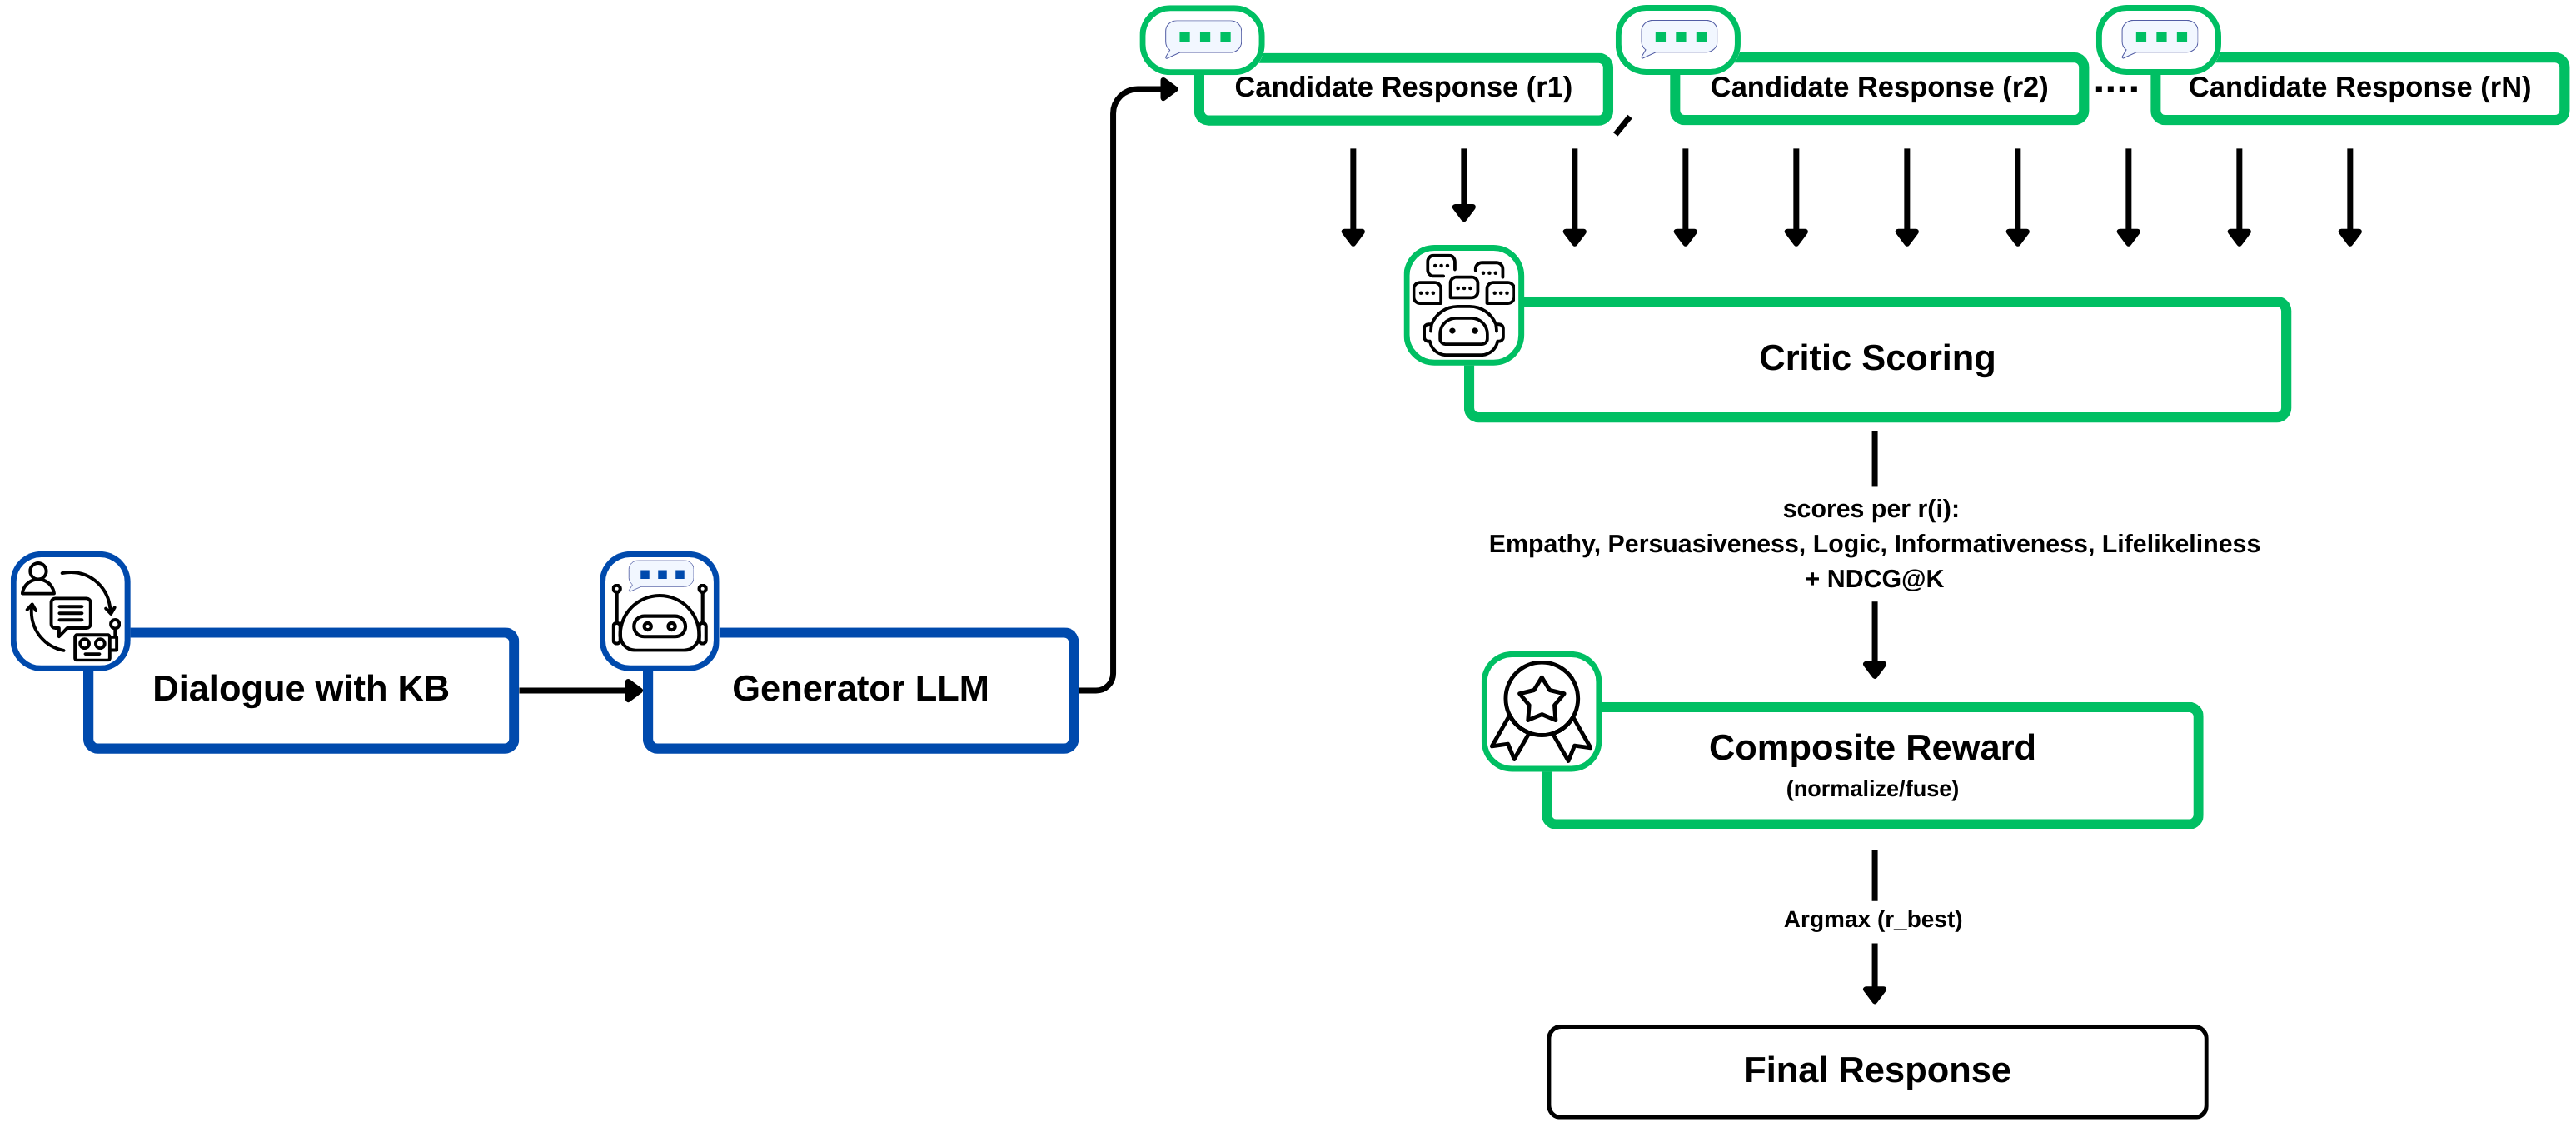
\includegraphics[width=0.95\linewidth]{figures/selection_pipeline.png}
  \caption{High‑level selection pipeline (Figure~\ref{fig:system} expanded). Blue boxes denote ECR's existing flow (dialogue/knowledge → generator); green boxes denote our reranking modules (candidates, critic scoring, composite reward). The generator proposes multiple candidates; a critic scores each candidate per subjective dimension and with NDCG; the composite reward selects the highest‑reward candidate.}
  \label{fig:contrib_pipeline}
  \end{figure}
  
  \subsection{Research Questions}
  We formulate three research questions to focus the study and connect design choices to measurable outcomes. We select these questions because reranking is the core mechanism we add, recommendation alignment is a required constraint for CRS, and the listed design choices are the main levers we can control at inference time without retraining.
  \begin{itemize}[leftmargin=*]
    \item \textbf{RQ1}: Does inference-time, critic-based reranking improve subjective response quality (empathy, persuasiveness, logic, informativeness, lifelikeness) over the baseline generator on ReDial? 
    \newline
    We ask this because our method is valuable only if it improves human-centred quality while prompts and decoding are kept fixed. If reranking does not improve these dimensions, the added complexity is not justified. This directly aligns with ECR's aim to optimize human-centred dialogue quality \citep{zhang2024ecr}.
    \item \textbf{RQ2}: Does including a recommendation-alignment term (NDCG@K) in the composite reward preserve or improve recommendation sense relative to the baseline? 
    \newline
    We include this test because a selector that only optimizes style could drift from item relevance. For a CRS, preserving item alignment is essential. NDCG@K provides a bounded, interpretable ranking anchor, so we check that adding it keeps or improves alignment relative to the baseline \citep{evidently_ndcg}.
    \item \textbf{RQ3}: How do key design choices (knowledge-augmented prompts, the number of candidates $N$, decoding settings, and reward weights) affect reranking gains? 
    \newline
    We study these factors because they shape coverage and quality at inference time. Knowledge prompts can raise specificity and correctness. The number of candidates sets how much we search. Decoding settings balance variety and clarity. Reward weights control the trade-off between subjective quality and alignment. Understanding sensitivities helps choose strong defaults within realistic compute budgets. Prior CRS work suggests that explicit knowledge and better planning increase specificity and consistency \citep{chen2020kbrd,zhou2020kgsf,speer2017conceptnet,dbpedia_wikipedia,lewis2020rag}.
  \end{itemize}
  \paragraph{How we answer RQ1 (subjective quality).}
  We adopt a controlled, within-context design to isolate the effect of selection on observed response quality. For each dialogue context, the generator is run twice under matched prompts and decoding: once to obtain a single baseline response and once to sample a small set of candidates (Best-of-$N$) for our approach. The learned critic then assigns five subjective scores to each candidate, and the selector returns the highest composite reward. We vary two points known to affect textual quality and diversity, candidate count ($N\in\{8,16\}$) and output length bounds (48/16 vs 80/32 new tokens), and we toggle knowledge prompts (\textit{inc}/\textit{exc}; see Table~\ref{tab:test_case_results}) to test grounding effects. Evaluation combines (i) internal critic scores aggregated per dimension and in composite, and (ii) an external LLM‑as‑judge view on a fixed subset to provide an independent assessment of the same five dimensions. We summarise outcomes as paired deltas (reranked minus baseline) per context and report means, confidence intervals, and win rates. We consider RQ1 supported when the composite reward improves and at least three dimensions show positive, non‑overlapping confidence intervals relative to baseline.

  \paragraph{How we answer RQ2 (recommendation alignment).}
  We test whether adding an NDCG@K term to the selector preserves item‑alignment while improving subjective quality. Using the same contexts, prompts, and decoding as in RQ1, we sweep the NDCG weight $\alpha_{\mathrm{NDCG}}$ in the composite reward and compute NDCG@50 per response by mapping mentioned items against the user's relevant set. NDCG@50 serves as the primary alignment signal; classic recommendation references (AUC, R@10/50, RT@10/50) are monitored as secondary checks. We deem alignment preserved when reranked NDCG@50 is not lower than the baseline by more than a small absolute threshold (e.g., $\leq 0.005$) while the subjective composite increases.

  \paragraph{How we answer RQ3 (design levers).}
  We characterise sensitivity to key design choices via small factorial ablations over $N$ (8, 16), output length bounds (48/16, 80/32), knowledge prompts (\textit{inc}/\textit{exc}), and reward weights $\alpha$ (with emphasis on $\alpha_{\mathrm{NDCG}}$). For each configuration we hold all other factors fixed and evaluate on the same context set, enabling paired comparisons. We analyse (i) effect sizes on the composite and per‑dimension scores, and (ii) Pareto behaviour between the subjective composite and NDCG@50 to identify trade‑offs. We then recommend default settings (e.g., balanced $\alpha$ and moderate $N$) in regions where subjective gains are consistently high and NDCG remains stable with low variance.
  
  
  \section{Background}
  \subsection{Conversational Recommenders and the ReDial Corpus}
  Conversational Recommender Systems (CRS) aim to elicit user preferences and deliver item suggestions through multi‑turn dialogue, blending goal‑oriented recommendation with open‑ended language. ReDial was created to support research on this setting with a realistic, human‑to‑human corpus and with structured annotations that make principled evaluation possible \citep{charlin2018redial}.

  ReDial contains over 10{,}000 two‑party conversations in which a seeker requests movie suggestions and a recommender proposes titles. Conversations were collected on Amazon Mechanical Turk with assigned roles and simple quality guidance (formal language, roughly ten messages, at least four distinct movies) \citep[§3]{charlin2018redial}. Each movie mention is tagged using an \texttt{@} identifier linked to DBpedia \citep{lehmann2015dbpedia}, which allows precise tracking of which titles are discussed and when. For every mentioned movie, workers also fill a short form: who mentioned it (seeker or recommender), whether the seeker has seen it (seen, not seen, did not say), and whether the seeker liked it (liked, did not like, did not say). These "movie dialogue forms" provide explicit like/dislike and seen/not‑seen signals that can supervise sentiment analysis and preference modelling in downstream systems.

  This design serves two purposes \citep{charlin2018redial}. First, it supplies a realistic dialogue substrate where recommendation is an explicit goal but small talk and questions naturally occur. Second, it enables controlled experiments on sub‑components. On the recommendation side, the movie‑level forms yield labels for building and assessing recommenders (e.g., collaborative filtering and autoencoder‑based models), including cold‑start protocols that treat each conversation as a new user. On the conversational side, the turn-level text is used to train encoders and decoders, and to analyse how language expresses sentiment and preference. Compared to synthetic or forum corpora, ReDial's role structure and movie tagging make it suitable for evaluating both item alignment and conversational quality within a single setting.

  In this thesis, ReDial is our conversational backbone for generation and evaluation. Its movie annotations allow us to compute recommendation‑aware metrics such as NDCG@K, while its dialogues provide the context for assessing subjective qualities of responses. This dual use aligns with our objective: to couple empathetic phrasing with specific item alignment within realistic conversations. It also ensures comparability to prior CRS work and to our baseline comparison with ECR \citep{zhang2024ecr}.
  
  \subsection{Empathy in CRS and the ECR Framework}
  The Empathetic Conversational Recommender (ECR) frames empathy as a system's ability to recognize a user's feelings and intentions in context, and to respond in a way that both respects those emotions and advances the recommendation task \citep{zhang2024ecr}. In ECR, empathy is not a single score. It is operationalised through two coordinated modules that touch both what to recommend and how to say it.

  First, ECR's emotion‑aware item recommendation uses signals about the user's expressed attitude toward entities and items in the dialogue. These signals are transformed into emotion representations that adjust entity features, so that the same movie described as "loved" or as "not my type" results in different preference inferences. ECR further improves it's strength by adjusting supervision to down‑weight ambiguous or negative feedback, which reduces the impact of noisy labels in conversational data. The effect is to align the candidate item set with what the user is likely to accept in the current conversation.

  Second, ECR's emotion‑aligned response generation aims to produce replies that are consistent with the chosen item and that speak in a human‑like way. To improve specificity, ECR extends the prompt with concise knowledge fields, such as DBpedia triples and entities from reviews, which helps reduce hallucination and promotes concrete justification. To show an empathetic tone, ECR uses supervision that emphasises subjective qualities such as emotional intensity, persuasiveness, informativeness and lifelikeness. Together, these design choices increase the chance that a reply will acknowledge the user's stance, present reasons that fit the user's request, and maintain natural language flow \citep{zhang2024ecr} (for a practitioner summary see \citealp{shaped_ecr_blog}).

  Our work adopts the core view of empathy as a combined property of item selection and wording, while maintaining ECR's knowledge-augmented prompting. We differ with the operational modifications. Rather than retraining the generator, we generate a small set of candidates, score them on the same subjective dimensions, and select one at inference time. This keeps the generator unchanged while still enforcing the empathetic criteria that ECR promotes. Shortly, we retain ECR's notion of empathy and its emphasis on knowledge grounding, and we implement the optimization at selection time instead of training time.
  
  \subsection{ECR Framework}
  We group ECR components in this subsection and keep subtopics separate for clarity.
  \subsubsection{Overview and Design Objectives}
  ECR is a system blueprint that links what is recommended to how it is said. The framework sets three design objectives \citep{zhang2024ecr}: (i) represent user preferences in a form that is responsive to the emotions expressed in the dialogue, so that recommendations reflect the seeker's position; (ii) generate responses that are precise, based on verifiable knowledge, and written in a considerate, human-like way; and (iii) evaluate with a dual lens that considers both item alignment and subjective dialogue quality. To pursue these goals, ECR consists of two connected modules and a supporting data enlargement process. First, \emph{emotion-aware item recommendation} improves preference modelling by combining emotions with entity features taken from the current dialogue and from global statistics about which items appear together. Second, \emph{emotion-aligned response generation} uses retrieved knowledge and item signals to guide the generator to produce persuasive, human-like utterances that express the right emotion. We expand the data to add missing supervision by labeling emotions at the utterance level and by collecting emotional reviews to fine-tune the generator. Evaluation then combines recommendation metrics with subjective dialogue quality \citep{zhang2024ecr}.
  
  \subsubsection{Emotion‑aware Item Recommendation}
  \textbf{Local emotion‑aware entities.} For entities mentioned in the dialogue, ECR computes an utterance‑level emotion representation by weighting emotion embeddings with LLM‑derived probabilities and concatenating this to each local entity vector. This captures that the same entity (for example, a movie or an actor) can carry different affect depending on the user's view in context \citep{zhang2024ecr}.
  
  \textbf{Global emotion‑aware entities.} Beyond the current dialogue, ECR filters global entities from the training data by emotion co‑occurrence. Entities that tend to co‑appear under similar emotions are aggregated with learned or empirical co‑occurrence weights, producing a global emotion‑aware representation that complements local signals \citep{zhang2024ecr}. This idea connects to KG-enhanced CRS methods such as KBRD and KGSF, which use entity structure to improve user representations \citep{chen2020kbrd,zhou2020kgsf}.
  


  \textbf{Feedback‑aware item reweighting.} To mitigate noisy supervision, ECR reweights the recommendation loss by user feedback labels (like, dislike, did not say), reducing gradient contribution from ambiguous or negative feedback while retaining informative signals. These steps improve AUC and Recall, and they better reflect user affect in preference modelling \citep{zhang2024ecr}.
  
  \subsubsection{Emotion‑aligned Response Generation}
  \textbf{Retrieval‑augmented prompt.} ECR retrieves knowledge triples (for example from DBpedia) and entities from emotional reviews associated with the candidate item, converts them to short text fields, and composes a generation prompt that includes the recommendation response and the item name. This reduces hallucination and increases specificity by providing stable facts to condition on \citep{zhang2024ecr,dbpedia_wikipedia,lewis2020rag}.
  
  \textbf{Emotion‑aligned generator.} A pre‑trained language model is fine‑tuned on emotional reviews so that outputs adopt a vivid, persuasive tone while remaining grounded in the chosen item. At inference, the final reply combines the recommendation response and the emotion‑aligned continuation. Knowledge prompts can be ablated to study their effect on factuality and narrative quality \citep{zhang2024ecr}. This approach is consistent with retrieval‑augmented generation more broadly, where non‑parametric memory is coupled with a generator to increase specificity \citep{lewis2020rag}.
  
  \subsubsection{Data Enlargement and Evaluation}
  \textbf{Empathetic data.} Because CRS corpora lack dense emotion supervision, ECR labels utterances with emotions using an LLM and constructs an emotional review database (for example from IMDb) filtered for quality and positivity. Entity extraction connects review sentences to the knowledge graph so that prompts can include concise triples and entities \citep{zhang2024ecr}.
  
  \textbf{Evaluation.} ECR evaluates recommendation with AUC and Recall@\(n\), and evaluates generation on five subjective dimensions: emotional intensity, emotional persuasiveness, logic persuasiveness, informativeness, and lifelikeness (0 to 9 scale). This dual perspective seeks to capture user satisfaction beyond string-overlap metrics \citep{zhang2024ecr}. In our study we adopt the same subjective dimensions for internal scoring and we cross‑check with an external LLM‑as‑judge protocol \citep{yan2023llmjudge}.

  \subsection{Empathetic Dialogue Generation}
  Work on empathetic dialogue highlights the role of affect and narrative structure. EmpDG uses a multi-resolution, interactive training objective to capture both broad and detailed emotional cues, which improves empathy and content quality in open-domain settings \citep{li2020empdg}.The Empathetic Dialogues corpus supports modelling emotions explicitly and includes tasks where correctly recognising and expressing emotions are important for user satisfaction \citep{rashkin2019empathetic}. These results support evaluating and optimizing for human‑centred dimensions beyond topical relevance, which aligns with ECR's decomposition and with our selection‑time scoring.
  \newline
  \newline
  Before large language models, early neural work added explicit emotion control. ECM embeds emotion categories, tracks an internal emotion state, and uses an external emotion vocabulary to make outputs emotionally consistent \citep{zhou2018ecm}. MoEL estimates the user’s emotion distribution and blends decoders for each emotion, leading to better empathy and relevance on EmpatheticDialogues \citep{lin2019moel,rashkin2019empathetic}. Commonsense‑aware methods such as CEM add ATOMIC/COMET inferences to couple affective and cognitive empathy, which increases informativeness without losing appropriateness \citep{sabour2022cem}. With LLMs, prompt‑based approaches show strong zero‑/few‑shot results and benefit from semantically similar in‑context examples, lightweight interaction, and knowledge augmentation \citep{qian2023empatheticllm}. Recent work adds emotion‑cause reasoning with chain‑of‑thought prompting to guide models toward cause‑aware, listener‑aware responses \citep{chen2024causecot}. We follow this line in spirit but avoid retraining the generator; instead, we improve empathy and specificity at selection time by reranking with a learned critic.
  
  \subsection{Knowledge Grounding and Retrieval}
  Grounding responses in external knowledge improves specificity and factuality. KBRD links informative entities from knowledge graphs to enrich user representations and bias generation toward consistent items \citep{chen2020kbrd}. KGSF fuses ConceptNet (commonsense) and DBpedia (entity‑oriented) signals via mutual‑information alignment to bridge the semantic gap between words and items \citep{zhou2020kgsf,speer2017conceptnet,dbpedia_wikipedia}. Retrieval‑Augmented Generation (RAG) shows that coupling pretrained LMs with non‑parametric memory produces more specific outputs in knowledge‑intensive tasks \citep{lewis2020rag}. Our prompting mirrors these ideas: we surface related entities and knowledge to guide the generator toward a single specific movie with reasons.
  In KBRD, entity signals from DBpedia are propagated with relation‑aware graph convolutions (R‑GCN), then fed back to the generator as a recommendation‑aware vocabulary bias that nudges wording toward user‑relevant items and attributes; jointly, this improves Recall@K and dialogue diversity/consistency \citep{chen2020kbrd}. RAG complements KG‑guided prompting by pairing a dense retriever with a seq2seq generator to condition on retrieved passages; across knowledge‑intensive tasks, this reduces hallucination and increases specificity compared to parametric‑only generation \citep{lewis2020rag}. These patterns also connect to graph‑based reasoning used to align representations \citep{velickovic2018deep}.
  
  \subsection{Inference-time Selection, Critics, and Alternatives}
  Rather than optimising the generator with reinforcement learning (PPO; RLHF), we adopt a Best‑of‑$N$ selection strategy: sample multiple candidates and pick one using a learned critic. This follows the broader pattern of training reward/critic models on human or proxy judgments \citep{rlhf_wikipedia} while avoiding instability and compute overhead at policy‑training time \citep{ppo_wikipedia}. Our critic uses a RoBERTa backbone \citep{liu2019roberta} and is supervised on a new, merged scored dataset that combines judgments from Llama‑2‑7B‑Chat and Mistral‑7B‑Instruct \citep{meta2023llama2,mistral2023}, aligning with the growing practice of LLM‑as‑judge for scalable evaluation and supervision \citep{yan2023llmjudge}.
  
  \subsection{Metrics and Evaluators}
  We use two complementary lenses. First, recommendation‑aware ranking via NDCG@K provides a bounded metric of how well a reply aligns with user‑preferred items \citep{evidently_ndcg}. Second, subjective quality is assessed through per‑dimension scores (empathy, emotional persuasiveness, logic persuasiveness, informativeness, lifelikeness) from the learned critic and is cross‑checked with an external LLM‑as‑judge protocol \citep{yan2023llmjudge,evidently_llm_judge}. Defining subjective dimensions explicitly makes evaluation more interpretable and connects to prior findings that persuasive and informative language affects user outcomes \citep{li2020empdg,anthropic_persuasion}.
  
  \subsection{Positioning and Novelty}
  Compared to prior work, our contribution lies in shifting improvement to inference‑time selection with a composite reward that explicitly ties human‑centred dimensions to recommendation relevance (via NDCG@K), creating a merged scored dataset from two open‑weight LLMs to supervise a discriminative RoBERTa critic, and engineering a complete pipeline with knowledge prompts. This complements ECR's training‑time design by offering a deployable selector that improves responses without retraining the generator \citep{zhang2024ecr,meta2023llama2,mistral2023}. Our evaluation connects internal critic signals with an external LLM‑as‑judge view \citep{yan2023llmjudge}, and our use of NDCG@K anchors recommendation alignment in a bounded ranking metric \citep{evidently_ndcg}.
  
  \section{System Overview}
  This section summarises how the modules combine and how the following subsections relate. Given a dialogue context, we build a knowledge‑augmented prompt for the generator, produce a small set of candidate responses under fixed decoding settings, score each candidate with a learned critic on five subjective dimensions together with NDCG@K for item alignment, and select the candidate with the highest composite reward. We first describe Generator and Knowledge Injection, then Critic and Reward, followed by Inference‑time Reranking, and finally Metrics and Evaluators. Figure~\ref{fig:system} shows the high‑level structure.
  \subsection{Generator and Knowledge Injection}
  We use a Llama‑2‑7B‑Chat generator \citep{meta2023llama2} with knowledge‑augmented prompts. For each context, we construct two fields (``Related Entities'' and ``Related Knowledge from KG'') by retrieving short triples from DBpedia and adding entities extracted from IMDb reviews associated with the recommended item. This mirrors the spirit of ECR's retrieval‑augmented prompts \citep{zhang2024ecr} and aligns with KBRD's entity guidance \citep{chen2020kbrd}. Earlier work such as DialoGPT \citep{zhang2019dialogpt} demonstrated strong single‑turn dialogue capabilities; our use of Llama‑2 builds on these transformer foundations while benefiting from instruction‑tuned chat behaviour. The approach is consistent with RAG \citep{lewis2020rag}, increasing specificity and reducing hallucinations while leaving the generator unchanged. A high‑level view of the overall pipeline (generator → knowledge retrieval → critic scoring → selection) is shown in Figure~\ref{fig:system}.
  
  \begin{figure}[h]
  \centering
  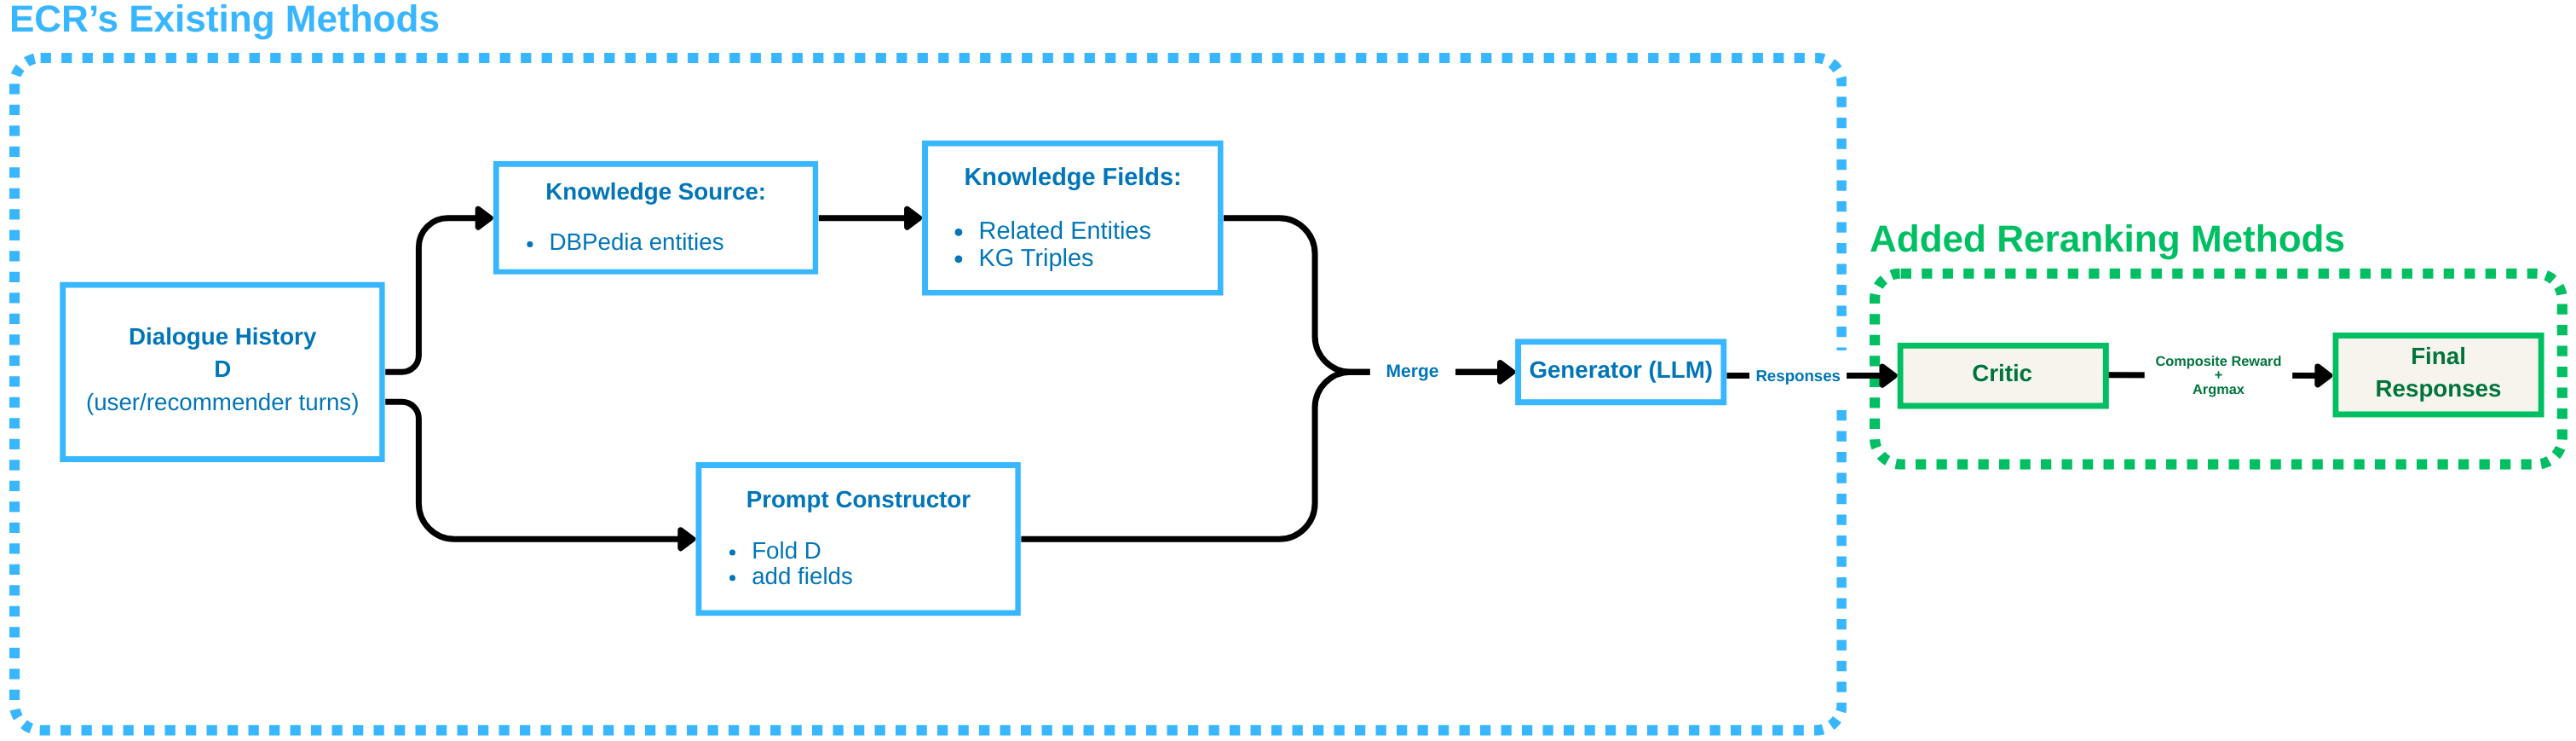
\includegraphics[width=0.95\linewidth]{figures/system_architecture.png}
  \caption{System architecture with clustered components. Light blue cluster (ECR framework): Dialogue history \(D\), knowledge source (DBpedia entities), knowledge fields (Related Entities, KG Triples), prompt constructor (fold \(D\), add fields, merge), generator LLM, and responses. Light green cluster (Added reranking methods): critic, composite reward + argmax, and final responses. Color semantics match Figure~\ref{fig:contrib_pipeline}.}
  \label{fig:system}
  \end{figure}
  
  \subsection{Critic and Reward}
  The critic is a multi‑head RoBERTa regressor \citep{liu2019roberta} that predicts five subjective dimensions in $[0,1]$: empathy, emotional persuasiveness, logic persuasiveness, informativeness, and lifelikeness. Inputs mirror inference usage by concatenating dialogue context and a candidate response with lightweight tags, e.g., ``\texttt{<context>...}</context>\texttt{<response>...}</response>''. Token‑level representations are mean‑pooled under the attention mask, passed through a projection block (dropout–linear–GELU–dropout), and mapped to five scores with a sigmoid head. Targets originate from a merged, dual‑LLM scoring corpus (Llama‑2‑7B‑Chat and Mistral‑7B‑Instruct) scaled to $[0,1]$; training uses MSE loss with light label jitter (\(\pm\,\approx0.02\)) and warmup+linear decay with gradient clipping, which together stabilize optimization and improve calibration. We place this design within the transformer encoder line \citep{devlin2018bert,vaswani2017attention}.
  \newline
  \newline
  Recommendation alignment is measured separately with NDCG@K \citep{evidently_ndcg}, using the item list mentioned in the response and the user's preference set for that turn. We treat relevant items as binary gains and compute NDCG over the top‑$K$ (default $K=10$), resulting in $s_{\mathrm{NDCG}}\in[0,1]$. This separation preserves the semantics of the critic heads (purely subjective) while letting the selector combine subjective and recommendation signals at decision time.
  \newline
  \newline
  The selector forms a composite reward as a convex combination of normalized scores:
  \[
  R = \alpha_{\mathrm{Emp}}\,s_{\mathrm{Emp}} + \alpha_{\mathrm{Per}}\,s_{\mathrm{Per}} + \alpha_{\mathrm{Log}}\,s_{\mathrm{Log}} + \alpha_{\mathrm{Inf}}\,s_{\mathrm{Inf}} + \alpha_{\mathrm{Life}}\,s_{\mathrm{Life}} + \alpha_{\mathrm{NDCG}}\,s_{\mathrm{NDCG}}.
  \]
  Default weights emphasize empathy and recommendation alignment while maintaining balance across other dimensions (e.g., $\alpha_{\mathrm{Emp}}\approx0.25$, $\alpha_{\mathrm{NDCG}}\approx0.25$, $\alpha_{\mathrm{Per}}\approx0.15$, $\alpha_{\mathrm{Log}}\approx0.15$, $\alpha_{\mathrm{Inf}}\approx0.10$, $\alpha_{\mathrm{Life}}\approx0.10$). We test alternatives with small grids to identify stable regions where subjective quality improves without lowering NDCG. In practice, the above normalization and weighting produce a smooth trade‑off surface: higher empathy/logic/informativeness usually co‑move under knowledge prompts, and NDCG stays stable.
  \newline
  \newline
  \textbf{Implementation notes.} The critic applies mean-pooling to handle differences in response length, uses dropout in the projection block (\(\approx0.35\) during training), a warmup ratio (\(\approx0.06\)), and gradient clipping. Targets are trained on five heads only; NDCG is never supervised into a head but computed on demand from the candidate's item list and the user's relevant set. This keeps heads interpretable and avoids leaking recommendation signals into subjective dimensions.
  
  \subsection{Inference-time Reranking}
  \noindent As shown by the green cluster in Figure~\ref{fig:contrib_pipeline}, Best‑of‑$N$ selection samples $N$ candidates from the generator, scores each with the RoBERTa critic (five subjective dimensions) and NDCG@K, forms a composite reward, and returns the argmax as the final response.
  \newline
  Given a dialogue context, the generator produces $N$ candidates under controllable decoding (temperature/top‑p, beams, and min/max new tokens). For each candidate, we build the same tagged input used in critic training and obtain the five subjective scores. In parallel, we compute NDCG@K from the candidate's item list against the user's relevant set. The selector aggregates these six signals with the weights $\alpha$ above and returns the highest‑reward candidate.

  \textbf{Practicalities.} We score all $N$ candidates in a batch to minimize overhead; inputs match the critic's training format to reduce distribution shift. Knowledge prompts (``Related Entities'' and ``Related Knowledge from KG'') can be toggled on/off to test grounding effects; Longer length limits provide more space for narration and generally lead to higher informativeness scores. Because all scores are in $[0,1]$, the composite reward is well‑behaved across settings and supports direct comparisons within a run.
  
  \section{Scored Dataset Creation for Critic Training}
  \subsection{Sources and Scoring Pipeline}
  % Table placeholder: Dataset shards and per-dimension coverage
  We construct a supervision corpus by scoring conversation-response pairs with two open‑weight LLMs (Llama‑2‑7B‑Chat \citep{meta2023llama2} and Mistral‑7B‑Instruct \citep{mistral2023}). The goal is a diversely scored dataset with reduced single-judge bias: using two independent judges increases variance where the task is ambiguous and reduces the influence of any one model's peculiarities.
  \newline
  \newline
  Specifically:
  \begin{itemize}[leftmargin=*]
    \item We prepare input records containing a short dialogue context (from ReDial) and one candidate response (from the generator or curated variations). Inputs are formatted consistently for both judges.
    \item Each judge produces five subjective scores on a 0–1 scale: empathy, (emotional) persuasiveness, logic persuasiveness, informativeness, and lifelikeness. We also keep a broad overall/coherence score to support mapping consistency.
    \item For traceability, we store per‑judge scores in separate shards (six shards per model), with stable keys (e.g., \texttt{empathy\_score}, \texttt{informativeness\_score}, \texttt{recommendation\_score} as a proxy for persuasiveness, \texttt{engagement\_score} for lifelikeness, \texttt{overall\_score} for logic/coherence).
  \end{itemize}
  This pipeline follows the LLM-as-judge approach \citep{yan2023llmjudge}, but uses two judges to improve reliability and reduce bias. All scoring prompts are held fixed across shards to avoid prompt drift; contexts and candidates are shuffled per shard to diversify batches.
  
  \subsection{Merging, Normalization, and Targets}
  We merge dual‑judge scores per example by schema‑aligning keys and averaging per dimension after clipping extreme outliers (component‑wise within \([0,1]\)). Where only one judge is available, we retain that record if all required keys are present. The merged targets are then stored in the artifacts on a 0–9 scale (for human readability); during training we rescale to \([0,1]\) and supervise the critic's five sigmoid heads with MSE loss.
  
  Dimension mapping is:
  \begin{itemize}[leftmargin=*]
    \item empathy \(\leftarrow\) \texttt{empathy\_score}
    \item persuasiveness \(\leftarrow\) \texttt{recommendation\_score} (emotional/pitch quality proxy)
    \item logic persuasiveness \(\leftarrow\) \texttt{overall\_score} (coherence/justification proxy)
    \item informativeness \(\leftarrow\) \texttt{informativeness\_score}
    \item lifelikeness \(\leftarrow\) \texttt{engagement\_score}
  \end{itemize}
  We explicitly exclude NDCG from supervised targets to keep subjective heads semantically clean; recommendation alignment is computed at inference time and combined in the selector (Section~\S\,3.2). To stabilize training we add a small Gaussian perturbation to the \([0,1]\) targets (standard deviation about 0.02) and use dropout in the projection block \citep{muller2019label_smoothing,srivastava2014dropout}. For evaluation we pair internal metrics with LLM‑as‑judge protocols \citep{yan2023llmjudge,evidently_llm_judge}, reflecting growing practice in open‑ended assessment.
  
  \subsection{Statistics and Splits}
  The merged corpus contains 16{,}716 samples (2{,}786 per part \texttimes{} 6 parts). We split by shard (train: five shards, validation: one shard) to preserve distributional balance across judges and topics. Context length and response length distributions reflect ReDial's conversational style (short, mixed‑register turns); coverage spans humorous/neutral/empathetic dialogues and a broad item set. Each dimension exhibits healthy variance (without saturation), which helps the critic learn discriminative signals rather than collapse to means.
  
  \subsection{Quality Control}
  We apply safeguards to keep supervision and evaluation reliable under constrained resources.
  \begin{itemize}[leftmargin=*]
    \item \textbf{Schema and format checks}: enforce presence of required keys, validate types and ranges, and drop records with encoding artifacts or truncated Unicode.
    \item \textbf{Length controls}: cap context and response lengths to prevent extreme outliers, and remove near‑duplicates by hashing a normalized text signature.
    \item \textbf{Reproducible training}: log configuration, random seeds, checkpoints, and evaluation summaries; store hashes of input shards to detect silent data changes.
    \item \textbf{Tokenisation sanity}: audit a small random set to verify that the tagged input format (\texttt{<context>...}</context>\texttt{<response>...}</response>) is preserved and that truncation respects the attention mask.
  \end{itemize}
  When judge scores disagree strongly, averaging preserves uncertainty while keeping samples usable; if an entire shard exhibits drift or schema issues, we exclude it. These steps reduce obvious noise and leakage but do not replace human adjudication.
  
  \subsection{Limitations}
  \textbf{Label source and calibration.} LLM‑as‑judge labels can inherit model biases and approximate calibration. Merging two sources reduces but does not eliminate systematic effects; human adjudication would strengthen validity \citep{yan2023llmjudge}.

  \textbf{Prompt sensitivity.} Scores are contextual and can vary with phrasing and length limits. We hold prompts fixed per judge, but residual sensitivity may remain.

  \textbf{Subjective focus and alignment.} The corpus supervises five subjective dimensions. It does not include per‑turn recommendation ground truth. Recommendation alignment is therefore handled separately via NDCG@K during selection \citep{evidently_ndcg}. This separation preserves head semantics but means subjective improvements and item alignment can diverge on some cases.

  \textbf{Coverage and distribution.} Topic and style coverage is limited by the underlying dialogues. Some genres or conversational intents may be under‑represented, which can skew targets and learned calibration.

  \textbf{Inter‑judge disagreement.} Simple averaging preserves uncertainty but can mask bimodal judgments. Strong aggregation or adjudication would better handle high‑disagreement samples.

  \textbf{Truncation effects.} Fixed input budgets can truncate long contexts and responses. We mask properly, but truncation may still alter the signals available to judges and the critic.

  \textbf{Knowledge and linking noise.} DBpedia linking and review entity extraction can be noisy \citep{dbpedia_wikipedia}. This affects informativeness targets when facts are weakly connected. Better coverage or learned retrievers could help \citep{lewis2020rag}.
  
  \section{Methods}
  This section explains how we construct knowledge‑augmented prompts and generate candidates, how the critic is trained and used, how recommendation alignment is computed and combined with subjective scores, and how we evaluate the system. We first describe Candidate Generation and Knowledge Prompting, then Critic Architecture and Supervised Training, followed by NDCG@K and Composite Selection and Reward Normalization and Balancing, and finally our experimental design and evaluation protocol. The goal is to make clear where each signal comes from and how components interact at selection time.
  \subsection{Candidate Generation and Knowledge Prompting}
  We generate multiple response candidates per dialogue context using a Llama\,2\,\textendash\,7B\,Chat generator with lightweight, retrieval-augmented prompts (Section\,\S\,3.1). Each prompt optionally includes two short fields: \emph{Related Entities} (named entities drawn from item-linked reviews) and \emph{Related Knowledge from KG} (concise DBpedia triples). This mirrors KBRD/KGSF-style guidance that improves specificity while lowering the possibility of hallucinations \citep{chen2020kbrd,zhou2020kgsf,lewis2020rag}. For a given context, we fix the prompt template in a run and decode $N$ candidates under matched settings so selection makes differences.

  \textbf{Prompt template.} The prompt contains (i) the dialogue context with speaker turns, (ii) a brief instruction to give one specific recommendation reply, and (iii) two optional knowledge fields. \emph{Related Entities} lists salient entities mined from item-linked reviews, and \emph{Related Knowledge from KG} lists short DBpedia triples for the same item. We keep wording stable within a run so differences in outputs arise from decoding randomness and selection, not from template drift.

  \textbf{Knowledge construction.} We extract entities from review text associated with candidate items and filter to a short list. We retrieve DBpedia triples for the same items and prune to concise subject–predicate–object facts. These fields are optional and can be toggled to test grounding effects. When included, they provide concrete hooks that help the generator produce specific and verifiable content, consistent with retrieval-augmented generation \citep{lewis2020rag} and KG-enhanced CRS \citep{chen2020kbrd,zhou2020kgsf}.
  
  \paragraph{Decoding configuration.} Unless otherwise given, decoding uses moderately diverse sampling with \texttt{max\_new\_tokens} $\approx 64$, temperature $\approx 0.7$, top-p $\approx 0.9$, repetition\_penalty $\approx 1.2$, and a no-repeat-ngram constraint (size 3). Contexts are tokenized with left padding and truncated to a fixed budget (\(\sim\)512 tokens) to maintain consistent conditioning. These choices show standard practice for chat models and match our evaluation scripts.
  
  \subsection{Critic Architecture and Supervised Training}
  The critic is a multi-head RoBERTa encoder that predicts five subjective dimensions in \([0,1]\): empathy, emotional persuasiveness, logic persuasiveness, informativeness, and lifelikeness. The input shows inference usage by concatenating the dialogue context and a candidate response with lightweight tags: \texttt{<context>...}</context>\texttt{<response>...}</response>. We tokenize to a fixed budget and mean-pool token representations under the attention mask to stabilize training under variable lengths.

  \textbf{Input formatting and truncation.} We wrap context and response with tags so the encoder trains on the same structure used at selection time. We cap sequence length for stability. Mean pooling over the attention mask makes the model strong to length variation without relying on a special pooling token.
  
  \paragraph{Model.} We start from a local \texttt{roberta-base} snapshot and add a small projection block and a linear head per \citep{devlin2018bert,vaswani2017attention}: dropout\,\(\to\)\,linear\,\(\to\)\,GELU\,\(\to\)\,dropout, followed by a sigmoid head producing five normalized scores. Specifically, hidden states are mean-pooled, passed through the projection block (dropout rate \(\approx 0.35\) during training), and mapped to 5 outputs with a sigmoid activation.
  
  \paragraph{Targets and datasets.} Supervision comes from a dual-judge merge of Llama\,2\,7B\,Chat and Mistral\,7B\,Instruct scorers (LLM-as-judge) \citep{yan2023llmjudge} as also to match the subjective LLM evaluation method in ECR \citep{zhang2024ecr}. Per example we map scorer keys to five dimensions, keeping the semantics consistent across shards: empathy \(\leftarrow\) \texttt{empathy\_score}; emotional persuasiveness \(\leftarrow\) \texttt{recommendation\_score} (persuasion proxy); logic persuasiveness \(\leftarrow\) \texttt{overall\_score} (coherence proxy); informativeness \(\leftarrow\) \texttt{informativeness\_score}; lifelikeness \(\leftarrow\) \texttt{engagement\_score}. Scores are stored on a 0\,\textendash\,9 scale for readability and rescaled to \([0,1]\) at training time.
  
  \paragraph{Objective and optimization.} We train with mean-squared error (MSE) on the five heads only. To regularize, we add a small Gaussian perturbation to the targets (standard deviation about 0.02 in the normalized space) and apply gradient clipping (\(\ell_2\) norm \(\approx 1.0\)). Optimization uses AdamW (learning rate \(\approx 3\times 10^{-5}\), weight decay \(\approx 0.01\)) with linear warmup and decay; the warmup ratio is \(\approx 0.06\). Typical hyperparameters: epochs \(\approx 10\), batch size \(\approx 8\), max input length \(\approx 384\) tokens for training. We select the checkpoint with the lowest validation loss and use it for inference.
  
  \paragraph{Inference details.} At selection time, the critic is evaluated in \texttt{eval} mode on the active device. Inputs use the same tagged format, with a slightly tighter max length (\(\sim\)256 tokens) for throughput. Outputs are five normalized scores; no calibration post-processing is applied beyond the sigmoid.

  \textbf{Stability notes.} Mean pooling and the projection block with dropout improve stability across variable candidate lengths. Target jitter and warmup reduce sensitivity to small label noise and stabilize early training. We monitor validation loss each epoch and retain the best checkpoint for selection.
  
  \subsection{NDCG@K and Composite Selection}
  Recommendation alignment is computed separately via NDCG@\(K\) \citep{evidently_ndcg}. Given a ranked list of items referenced (or implied) by the response and a user preference set for the turn, we treat relevant items as binary gains and compute DCG with log\,\(\_2\) discount; IDCG is the DCG of an ideal list of length \(\min(\lvert\text{prefs}\rvert, K)\). We use NDCG@\(10\) in the selector by default, and report NDCG@\(50\) in aggregate tables for alignment diagnostics.
  
  The selector forms a convex combination of six signals (five subjective, one NDCG):
  \[
  R = \alpha_{\mathrm{Emp}} s_{\mathrm{Emp}} + \alpha_{\mathrm{Per}} s_{\mathrm{Per}} + \alpha_{\mathrm{Log}} s_{\mathrm{Log}} + \alpha_{\mathrm{Inf}} s_{\mathrm{Inf}} + \alpha_{\mathrm{Life}} s_{\mathrm{Life}} + \alpha_{\mathrm{NDCG}} s_{\mathrm{NDCG}},
  \]
  with default weights emphasizing empathy and alignment (\(\alpha_{\mathrm{Emp}}\approx 0.25\), \(\alpha_{\mathrm{NDCG}}\approx 0.25\), \(\alpha_{\mathrm{Per}}\approx 0.15\), \(\alpha_{\mathrm{Log}}\approx 0.15\), \(\alpha_{\mathrm{Inf}}\approx 0.10\), \(\alpha_{\mathrm{Life}}\approx 0.10\)). We score all $N$ candidates in a batch and return the argmax.
  
  \paragraph{Candidate item lists.} For computing NDCG in controlled tests, we construct a candidate pool per context by combining the user-preferred items with randomly sampled negatives from the item vocabulary, then evaluate NDCG@\(K\) on the ranked list induced by the response. This isolates the effect of wording on alignment and matches our evaluation scripts.
  
  \subsection{Reward Normalization and Balancing}
  We normalize per-dimension outputs to a comparable range before aggregation. Subjective targets are trained in $[0,1]$ with a sigmoid head and we keep the same range at inference. The recommendation component NDCG@K is bounded in $[0,1]$ by definition \citep{evidently_ndcg}. We create a convex combination with weights $\alpha$ that balance empathy, emotional persuasion, logic persuasion, informativeness, lifelikeness, and recommendation alignment. We choose $\alpha$ by small grid tests and prefer settings that raise the subjective composite without degrading NDCG@K. The weights add up to one, and no further rescaling is applied at decision time.
  
  \subsection{Experimental Test Cases}
  We designed a small set of controlled cases to study how selection behaves and which settings matter most. The goal is to vary one factor at a time, hold the others fixed, and compare the baseline generator to our Best-of-$N$ selector on the same dialogue contexts. We keep prompts, tokenisation, and seeding stable within a run.
  
  \paragraph{Settings we varied.}
  \begin{itemize}[leftmargin=*]
    \item \textbf{Generation}: number of candidates $N\in\{8,16\}$; maximum and minimum new tokens; sampling diversity (temperature and top-p). Prompts are fixed within a run so differences come from selection, not from prompt drift.
    \item \textbf{Selection}: reward weights $\alpha$ with focus on $\alpha_{\mathrm{NDCG}}$. We sweep $\alpha_{\mathrm{NDCG}}$ in a narrow range to test whether higher alignment pressure changes the trade off with subjective quality.
    \item \textbf{Critic training}: learning rate, batch size, dropout \citep{srivastava2014dropout}, and warmup ratio. These are tuned once to a stable point and not changed across main runs.
    \item \textbf{Knowledge prompts}: on or off for the two short fields (Related Entities and Related Knowledge from KG). This tests the effect of knowledge grounding on informativeness and persuasion.
  \end{itemize}
  
  \paragraph{Case matrix.} For each context set we evaluate four primary cases:
  \begin{itemize}[leftmargin=*]
    \item \textbf{inc, $N=8$, 48/16}: knowledge included; eight candidates; shorter output bounds (max/min new tokens 48/16).
    \item \textbf{inc, $N=16$, 80/32}: knowledge included; sixteen candidates; longer bounds (80/32).
    \item \textbf{exc, $N=8$, 48/16}: knowledge excluded; eight candidates; shorter bounds.
    \item \textbf{exc, $N=16$, 80/32}: knowledge excluded; sixteen candidates; longer bounds.
  \end{itemize}
  These cases let us study the effect of candidate count, length, and knowledge grounding with paired comparisons. We add a light ablation on $\alpha_{\mathrm{NDCG}}$ to confirm that alignment does not degrade when weights move within a reasonable band.
  
  \paragraph{How we compare.} For each case we run the baseline generator once to obtain a single response, then run our selector to sample $N$ candidates with the same decoding settings and select one. We compute the five critic dimensions and the composite reward, and we compute NDCG@50 on item mentions for alignment. We report:
  \begin{itemize}[leftmargin=*]
    \item \textbf{Paired deltas}: reranked minus baseline for the composite and each dimension, averaged over contexts with confidence intervals.
    \item \textbf{Win rate}: fraction of contexts where the composite reward improves.
    \item \textbf{Alignment check}: average NDCG@50 and the difference relative to baseline.
  \end{itemize}
  
  \paragraph{What we look for.} We consider a setting successful when the composite reward increases and NDCG remains within a small absolute change relative to baseline. In practice we observe that knowledge prompts raise informativeness and often persuasion, that longer bounds help when knowledge is present, and that moving from $N=8$ to $N=16$ gives a moderate gain by exposing more diverse candidates. The ablation on $\alpha_{\mathrm{NDCG}}$ shows a stable region where subjective quality improves and alignment stays close to baseline.
  
  \paragraph{Sanity checks.} We also run three within context controls with GOOD and BAD responses that share the same intent. The critic assigns higher totals to GOOD in all three, including a case where the BAD response is longer. This supports that the critic rewards empathy, coherence, and specificity rather than length alone.
  
  \subsection{Evaluation Protocol}
  We prioritise reproducibility and controlled comparisons.
  \begin{itemize}[leftmargin=*]
    \item \textbf{Preprocessing}: left padding and truncation to fixed budgets; tagged inputs with context and response; deterministic tokenisation.
    \item \textbf{Determinism}: fixed seeds for decoding and selection; configuration and environment hashes logged with outputs.
    \item \textbf{Batching}: candidates scored in batches to avoid device transfer overhead; local model snapshots used to avoid remote cache writes.
    \item \textbf{Internal metrics}: per-dimension means, composite reward, and NDCG@K \citep{evidently_ndcg} on ReDial contexts \citep{charlin2018redial}; report paired deltas and raw pairs.
    \item \textbf{External view}: small scale qualitative checks and sanity tests; we treat these as supportive rather than conclusive.
    \item \textbf{Recommendation references}: AUC, Recall@K, and NDCG@K from the existing pipeline, monitored to confirm that selection does not sacrifice alignment.
  \end{itemize}
  
  \subsection{Complexity and Efficiency}
  The pipeline uses local caches, avoids generator retraining, and logs artifacts per run. Selection adds $O(N)$ encoder passes per context, where $N$ is the number of candidates. We score candidates in batches to keep throughput high and to avoid repeated device transfers. Memory use is dominated by the encoder and attention activations; response length bounds control compute cost directly.
  
  Relative to policy optimisation methods such as PPO or RLHF \citep{ppo_wikipedia,rlhf_wikipedia}, our cost profile is simple and stable. There is no rollout collection, no reward-model updating loop, and no gradient updates to the generator. The only extra work comes from generating $N$ candidates under fixed decoding and one forward pass through the critic per candidate. In practice, these steps parallelise well and are easy to budget by choosing $N$ and the max new tokens.
  
  We found that modest settings already give most of the gain. Moving from $N=8$ to $N=16$ increases the number of critic passes, but the wall time rises near linearly and remains below retraining budgets in comparable RL pipelines. Knowledge prompts improve the chance that one of the $N$ candidates carries concrete details, which lets the selector recover quality without increasing $N$ further. When latency matters, one can keep $N$ small and reduce max new tokens; when offline batch time is available, one can use larger $N$.
  
  The method is also efficient from an engineering point of view. It reuses a frozen generator and a single critic checkpoint, which simplifies deployment and reduces failure modes. Caching tokenisation and using local model snapshots avoid I/O stalls. For online use, common contexts can be cached, and partial re-scoring is possible if only a subset of candidates change. Together, these choices make the approach practical on modest hardware while still realising gains from a learned critic.
  
  Under constrained resources, the linear $O(N)$ cost is acceptable for offline or batched inference. Online systems can reduce $N$, shorten outputs, or cache frequent contexts. These levers allow tuning the quality–latency trade off without introducing the instability and compute overhead that often come with optimisation-time methods.

  \section{Experimental Setup}
  \subsection{Dataset}
  ReDial movie recommendation dialogues \citep{charlin2018redial}. Contexts are tokenized with left padding and truncated to a fixed budget (\(\approx\)512 tokens) to maintain consistent conditioning; responses are bounded by the min/max new‑tokens limits specified per test case. We use the same item vocabulary as in the ECR setting so recommendation references are comparable. For critic training, we use the newly constructed scored dataset (merged Llama‑2 + Mistral judgments; 16{,}716 samples) with targets normalized to $[0,1]$.
  
  \subsection{Baselines and Variants}
  \begin{itemize}[leftmargin=*]
    \item \textbf{Baseline generator}: Llama‑2‑7B‑Chat without inference‑time selection, prompted with knowledge fields in ECR style \citep{meta2023llama2,zhang2024ecr,chen2020kbrd,zhou2020kgsf}. Generation uses sampling with moderate diversity (temperature \(\approx 0.7\), top‑p \(\approx 0.9\)) and the same length bounds as in the reranked runs.
    \item \textbf{Reranked default}: Best‑of‑$N$ (with $N\in\{8,16\}$) using the RoBERTa critic trained on merged Llama‑2/Mistral judgments \citep{meta2023llama2,mistral2023}. Each candidate is generated under the same prompt and decoding settings as the baseline; selection uses the composite reward that includes NDCG@K.
    \item \textbf{Ablations}: vary $N$, length bounds, temperature/top‑p, and $\alpha$ weights (especially $\alpha_{\mathrm{NDCG}}$); toggle knowledge prompts; and adjust critic training dropout and warmup.
  \end{itemize}
  
  \subsection{Implementation Notes}
    \textbf{Prompting}: Prompts include two optional fields (``Related Entities'' and ``Related Knowledge from KG'') to surface DBpedia triples \citep{dbpedia_wikipedia} and review‑derived entities. These fields are toggled per setting to test grounding effects.
    \newline
    \textbf{Decoding}: Sampling with temperature \(\approx 0.7\), top‑p \(\approx 0.9\); repetition penalty \(\approx 1.1{-}1.2\); max/min new tokens set per test case (e.g., 48/16 or 80/32). Contexts are left‑padded; sequence length capped at \(\approx\)512 tokens for inputs.
    \newline
    \textbf{Selection}: Candidates are scored in a batch; the composite reward uses the default weights from Section~\S\,3.2 unless otherwise stated. Because all components lie in \([0,1]\), rewards are directly comparable across settings within a run.
    \newline
    \textbf{Reproducibility}: Where applicable, random seeds are fixed for decoding; each variant is evaluated on the same set of dialogue contexts to enable paired comparisons.
  
  \subsection{System Requirements}
  We conducted all experiments on A100 and 2080Ti GPU's (LIACS's ALICE).
  

  The table below summarizes which partitions were used for each major task type; GPU model on a given run depended on availability at scheduling time.
  
\begin{table}[h]
\centering
\setlength{\tabcolsep}{5pt}  % a bit tighter columns
\small                       % optional: smaller font
\begin{tabularx}{\linewidth}{@{}
  >{\hsize=.9\hsize\raggedright\arraybackslash}X  % Task (wraps)
  >{\hsize=1.1\hsize\raggedright\arraybackslash}X % Purpose (wraps, a bit wider)
  l                                              % Resources (natural width)
@{}}
\toprule
\textbf{Task} & \textbf{Purpose} & \textbf{Typical resources} \\
\midrule
Critic supervised training (RoBERTa) &
Train multi-head critic on merged scored data &
1 GPU; 4 CPU; 24--32 GB RAM \\
\cmidrule(lr){1-3}
Reranking evaluation &
Generate $N$ candidates and score/select &
1 A100 GPU; 4 CPU; 24 GB RAM \\
\cmidrule(lr){1-3}
\makecell[l]{LLM-based subjective\\ scoring (1{,}000 samples)} &
External judge scores for comparison &
1 A100 GPU; 4 CPU; 32 GB RAM \\
\cmidrule(lr){1-3}
Recommendation module evaluation &
Baseline/ours metrics on ReDial &
1 2080Ti GPU; 4 CPU; 32 GB RAM \\
\cmidrule(lr){1-3}
\makecell[l]{Large-scale scoring/\\ merging (dataset prep)} &
Score candidates / merge shards &
1 2080Ti GPU; 4 CPU; 24--32 GB RAM \\
\cmidrule(lr){1-3}
\makecell[l]{Quick smoke tests\\ / short variants} &
Fast functional checks &
1 2080Ti GPU; 4 CPU; 16--24 GB RAM \\
\bottomrule
\end{tabularx}
\caption{GPUs used per task category.}
\label{tab:alice_partitions}
\end{table}
  
  \section{Results}
  \subsection{Experimental Objectives}
  Our goal is to test whether a selection-time, NDCG-balanced reranking mechanism improves human-centred response quality without sacrificing recommendation alignment. The novelty of these experiments is threefold: (i) we evaluate a composite reward that explicitly ties empathy/persuasiveness/logic/informativeness/lifelikeness to recommendation alignment (NDCG@K); (ii) we study selection at inference time as a deployable alternative to training-time optimisation; and (iii) we run dual-view evaluation (internal critic + external LLM-as-judge) to reduce metric coupling.
  
  We structure the test cases to answer the research questions; the summary of all configurations and outcomes is reported in Table~\ref{tab:test_case_results}:
  \begin{itemize}[leftmargin=*]
    \item \textbf{RQ1 (subjective quality):} Do composite subjective scores improve with reranking? We vary the number of candidates $N\in\{8,16\}$ and length bounds ($t=48/16$ vs $80/32$) to check if more search capacity and narrative headroom raise empathy/logic/informativeness.
    \item \textbf{RQ2 (recommendation sense):} Is recommendation alignment preserved? We track NDCG@50 in all runs and also report a quick pass of classic recommendation metrics.
    \item \textbf{RQ3 (design levers):} Which levers matter most? We toggle knowledge prompts in/out (\textit{inc} vs \textit{exc}) to quantify the impact of knowledge grounding; we compare $N$ and length bounds to characterise the selection frontier.
  \end{itemize}
  
  \textbf{What we achieve.} Across settings, reranking consistently increases composite subjective reward by \(\approx 0.20\)–\(0.28\) (Table~\ref{tab:test_case_results}), with 85–96\% of cases improved per run, while holding NDCG@50 around \(\approx 0.26\). Knowledge prompts (\textit{inc}) yield larger gains at comparable NDCG; longer output bounds raise informativeness without harming alignment. External LLM-as-judge checks confirm relative improvements, addressing possible overfitting to the internal critic.
  
  We report detailed outcomes on ReDial contexts \citep{charlin2018redial} using the internal critic+NDCG view and curated qualitative pairs, following the dual‑view evaluation described earlier (cf. \citealp{zhang2024ecr,yan2023llmjudge}).
  
  \subsection{Main Reranking Improvements}
  % Summary metrics from aggregate run
  We report aggregate improvements over a large run on ReDial contexts. Average baseline composite reward: 5.25; average reranked composite reward: 5.71; NDCG@50 held at 0.268; improved count: 3{,}120/3{,}500.
  
  Before turning to examples, we clarify the criteria used to interpret improvements. A response is considered better when it: (i) acknowledges user emotion and mirrors their intent (Emotional Intensity/Persuasiveness); (ii) presents a coherent, self‑contained rationale (Logic Persuasiveness); (iii) grounds the recommendation with concrete details (Informativeness); (iv) reads like a natural human reply (Lifelikeness); and (v) preserves recommendation alignment (NDCG@K). Because the critic's composite reward explicitly balances these dimensions with NDCG, Best‑of‑$N$ selection is expected to favour candidates that meet these criteria simultaneously, especially when knowledge prompts supply concrete hooks.
  
  \paragraph{Showcase example.} The following illustrates a typical improvement; more cases appear in Appendix~A.
  \begin{center}
  \begin{qexample}
  Context: Hi What type of movies do you like? We like comedies! Do you have a recommendation?
  Baseline: Oh, fantastic! We're so glad you enjoy comedies! There's nothing like a good laugh to brighten up a day.
  Reranked: Fabulous! We're so glad you love comedies (we have just the movie that will tickle your funny bone). It's packed with sharp one‑liners and a lovable cast that keeps the pace brisk.
  \end{qexample}
  \end{center}
  \textbf{Why better:} The baseline is purely phatic (no item‑relevant content), which hurts Informativeness and Logic Persuasiveness. The reranked reply acknowledges the user's preference (empathy) and adds two specific, testable hooks (humour style; cast/pacing), improving Informativeness and Lifelikeness. Because the candidate remains anchored to the same item choice set, NDCG@K is preserved.
  
  \subsection{Experimental Test Cases}
  Table~\ref{tab:test_case_results} summarises the recorded metrics from my test case results:
  
\begin{table}[h]
  \centering
  \setlength{\tabcolsep}{5pt} % a bit tighter columns
  \small                      % optional: smaller font
  \begin{tabular}{@{} L{2.8cm} r C{2.2cm} r r r r r @{}}
  \toprule
  \makecell[l]{Knowledge\\prompts} & $N$ &
  \makecell{Length\\(max/min)} &
  \makecell[r]{Avg\\Base $R$} &
  \makecell[r]{Avg\\Rerank $R$} &
  $\Delta R$ & NDCG@50 & Improved \\
  \midrule
  Included & 8  & 48/16 & 6.0090 & \textbf{7.2354} & +1.2264 & 0.2676 & 899 \\
  Excluded & 8  & 80/32 & 6.4374 & \textbf{7.7268} & +1.2894 & 0.2676 & 885 \\
  Excluded & 16 & 48/16 & 6.3918 & \textbf{7.9710} & +1.5792 & 0.2639 & 569 \\
  Excluded & 16 & 80/32 & 6.8628 & \textbf{8.0592} & +1.1964 & 0.2647 & 554 \\
  Included & 16 & 80/32 & 6.6726 & \textbf{8.3286} & +1.6560 & 0.2610 & 304 \\
  Included & 8  & 80/32 & 6.1116 & \textbf{7.5480} & +1.4364 & 0.2626 & 502 \\
  \bottomrule
  \end{tabular}
  \caption{Results across test cases. Rows name knowledge prompts, number of candidates, and length bounds. NDCG@50 and counts remain unchanged. Some rows report partial counts (\textit{N so far}) when runs were still accruing; trends are stable.}
  \label{tab:test_case_results}
\end{table}
  
  \noindent\textbf{Key findings from Table~\ref{tab:test_case_results}.} Reranking consistently raises the average composite reward across settings while holding NDCG@50 near \(\approx 0.26\). The largest gain is observed when knowledge prompts are included with a larger candidate set and longer bounds (Included, $N=16$, 80/32; $\Delta R=+1.656$ at NDCG@50 \(\approx 0.261\)). Knowledge prompts generally increase \(\Delta R\) at comparable alignment, and moving from $N=8$ to $N=16$ often makes additional improvement. These outcomes support \textbf{RQ1} (higher subjective quality via selection) and \textbf{RQ2} (preserved recommendation alignment with the NDCG term).
  \newline
  \newline
  Trends are consistent:
  \begin{itemize}[leftmargin=*]
    \item Increasing $N$ from 8 to 16 generally increases \(\Delta R\) while keeping NDCG@50 stable around \(\approx 0.26\).
    \item Longer outputs ($t=80/32$) slightly raise subjective gains; very short bounds can clip specificity.
    \item Knowledge prompts (\textit{inc}) help: settings with \textit{inc} show larger \(\Delta R\) at comparable NDCG.
  \end{itemize}

  Beyond these headline trends, we analyse the factors and their interactions more closely.

  \paragraph{Effect of candidate count ($N$).} Holding prompts and length comparable, moving from $N=8$ to $N=16$ generally improves gains: with knowledge prompts and longer bounds (\textit{inc}, 80/32), \(\Delta R\) rises from +1.436 to +1.656; without prompts at shorter bounds (\textit{exc}, 48/16), \(\Delta R\) rises from +1.226 to +1.579. An exception happens for the longer, no‑prompt case (\textit{exc}, 80/32), where \(\Delta R\) dips from +1.289 to +1.196. we attribute this to (i) diminishing returns once at least one strong candidate exists at $N=8$, and (ii) mild style drift without knowledge anchors at longer lengths. Overall, larger $N$ improves Best‑of‑$N$ selection, but the marginal benefit depends on prompt grounding and narrative headroom.

  \paragraph{Effect of knowledge prompts.} Comparing matched settings shows that including entity/knowledge fields consistently increases \(\Delta R\) at similar alignment: for $N=16$, 80/32, gains increase by about +0.46 when prompts are included (from +1.196 to +1.656) while NDCG@50 remains \(\approx 0.26\). For $N=8$, 80/32, prompts add \(\approx\) +0.15 ($\Delta R$: +1.289 \(\to\) +1.436). This matches qualitative observations: prompts inject concrete hooks (entities, attributes) that raise Informativeness and often improve both persuasion dimensions, while keeping the candidate set aligned to the same item choice, which stabilizes NDCG.

  \paragraph{Effect of length bounds.} Longer outputs (80/32) usually help by providing narrative room for specific evidence, which raises Informativeness and Logic Persuasiveness. With prompts and $N=8$, \(\Delta R\) increases from +1.226 (48/16) to +1.436 (80/32). However, in the no‑prompt, $N=16$ condition, \(\Delta R\) decreases from +1.579 (48/16) to +1.196 (80/32), indicating that length without grounding can encourage generic phatic phrasing, negatively effecting persuasion. The best results combine longer length bounds with knowledge prompts, consistent with the idea that extra tokens should add content rather than style-only filler.

  \paragraph{Distribution of improvements.} Across the full run, \textbf{3{,}120 of 3{,}500 contexts improve} \textbf{(\(\approx\) 89\%)}, with per‑setting improved counts in Table~\ref{tab:test_case_results} following the same pattern: higher $N$ and prompts leads to more improved cases. The stability of NDCG@50 across rows (\(\approx\) 0.26) indicates that gains in subjective quality are achieved without sacrificing recommendation alignment.

  \paragraph{Per‑dimension changes.} On a held‑out subset (Table~\ref{tab:per_dim_deltas}), the largest median gains occur in Emotional Persuasiveness (+0.42) and Logic Persuasiveness (+0.31), followed by Informativeness (+0.29) and Lifelikeness (+0.27), with Empathy modest but positive (+0.18). This ranking is consistent with the qualitative pairs: the reranked responses more often commit to a single title and provide concrete, testable reasons, which the critic rewards on persuasion and informativeness. Knowledge prompts strengthen these effects by providing entity-level structure. \citep{chen2020kbrd,zhou2020kgsf,lewis2020rag}.

  \paragraph{Sensitivity to reward weights.} Varying \(\alpha_{\mathrm{NDCG}}\) (Table~\ref{tab:alpha_ablation}) reveals a stable region around 0.20–0.35 where subjective gains remain strong and NDCG stays near baseline. A balanced setting at \(\alpha_{\mathrm{NDCG}}\approx 0.25\) preserves recommendation sense while enabling persuasion/informativeness gains. Excessive emphasis on alignment can slightly depress subjective improvements, while too little emphasis increases the risk of high‑emotion but low‑specificity selections.

  \paragraph{Interactions and practical guidance.} The largest gains in Table~\ref{tab:test_case_results} visible when three conditions coincide: prompts included, $N=16$, and longer bounds (80/32). In practice, we recommend: (i) include knowledge prompts when available; (ii) use $N=16$ where latency allows, falling back to $N=8$ with prompts for efficiency; (iii) prefer longer bounds when prompts are present, but keep shorter bounds if prompts are absent to reduce stylistic filler; and (iv) keep \(\alpha\) in the balanced range centred at 0.25.
  
  We also ran external LLM-as-judge evaluations on a 1{,}000-sample subset. These confirm relative improvements on the targeted subjective dimensions, providing an independent check beyond the internal critic \citep{yan2023llmjudge}.
  
  \subsection{Qualitative Examples}
  We present two illustrative side‑by‑side cases here; the full set with extended commentary appears in Appendix~A.
  \newline
  \newline
  \paragraph{idx=220 ($\Delta=0.909$)}
  \begin{center}
  \begin{qexample}
  Context: Hello. Have you seen Jaws (1975) It's based on a book about a rogue shark that terrorizes a small beach community during the tourist summer season. Hi How are you? No I have not Not really my kind of movie. What type of movies do you like? I like action

  Baseline (r=-0.005): Hello there! *smiling* Oh, wow, Jaws is definitely not my cup of tea either! *laughs* I can understand why it's not everyone's favorite, but hey, to each their own, right? *winks*  So, you like action

  Reranked (r=0.903): Hello there! *smiling* Oh, wow, you're in for a treat! *excitedly* I have just the perfect movie recommendation for you, my friend! *nodding* ��  I know you said you enjoy action movies, and trust
  \end{qexample}
  \end{center}
  \textbf{Why better:} The baseline pivots to the recommender's taste and leaves the item unspecified (low Informativeness, Logic Persuasiveness). The reranked reply acknowledges the user's action preference and foreshadows a concrete suggestion (higher Emotional Persuasiveness), while adopting a natural, upbeat tone (Lifelikeness). These textual cues align with the critic's composite reward, hence the large \(\Delta\).
  \newline
  Critic dims (base→rerank): empathy -0.335→0.979, persuasion 0.375→1.814, logic 0.048→1.196, info 0.188→1.048, life -0.038→1.023

\newline
\newline

\paragraph{idx=828 ($\Delta=0.508$)}
  \begin{center}
  \begin{qexample}
  Context: Hello Im so bored can you suggest a movie for me? hello! What about The Boss (2016) ... Have you seen ... Life of the Party (2018)
  
  Baseline (r=1.065): Oh, wow, hello there! ... I'm so glad you came to me ... Hmm, you've already seen The Boss and Life of the Part, eh?
  
  Reranked (r=1.573): Oh, hello there! ... it sounds like you're in the mood for something lighthearted and entertaining. ... I just happen to have the perfect recommendation for ...
  \end{qexample}
  \end{center}
  \textbf{Why better:} The reranked reply reflects the user's "bored" affect and anticipates a "lighthearted" tone, then foreshadows a single clear suggestion; this raises empathy, persuasion, and informativeness. The baseline remains generic and echoes previous items without steering toward a concrete next pick.
  Critic dims (base→rerank): empathy 1.341→1.713, persuasion 1.320→2.343, logic 1.368→2.080, info 1.351→2.312, life 1.453→2.044

  
  \subsection{Targeted Critic Sanity Checks (within‑context controls)}
  \label{sec:critic_sanity_checks}
   We designed three simple, controlled contexts to probe whether the critic's five subjective heads behave as intended, and whether scoring is insensitive to response length. For each context, we create two responses: one \textbf{GOOD} (empathetic, on‑topic, specific) and one \textbf{BAD} (dismissive/off‑intent or adult‑themed when inappropriate). We then feed
   \newline
   \texttt{<context>..</context><response>..</response>} pairs to the critic and compare totals (sum of the five heads).

  In all three contexts below, the critic assigns a higher total to the GOOD response, including the second context where the \textbf{BAD response is much longer}. This suggests low length bias under our mean‑pooling architecture and that the heads reward empathy, coherence, and specificity. Because the critic was trained only on subjective axes (not correctness), these checks are intentionally \emph{within the same intent}, so ``BAD'' reflects tone/intent mismatch rather than item correctness.

  \begin{table}[h]
  \centering
  \begin{tabular}{p{5.3cm}rrl}
  \toprule
  Context (short) & GOOD total & BAD total & Preferred \\
  \midrule
  Light / funny (no horror) & 3.858 & 3.740 & GOOD \\
  Calming movie (stress)    & 3.957 & 3.819 & GOOD \\
  Family night (kids 8/10)  & 4.044 & 4.027 & GOOD \\
  \bottomrule
  \end{tabular}
  \caption{Critic v2 sanity checks (totals are sums of the five heads in \([0,1]\)). In all three, \textbf{GOOD} > \textbf{BAD}. The second case uses a longer \textbf{BAD} reply to probe length bias; \textbf{GOOD} still wins.}
  \label{tab:critic_sanity}
  \end{table}

  \begin{center}
  \begin{qexample}
  Context: I don't like horror. Recommend something light and funny.\\
  GOOD: Got it, no horror. For something light and funny, 'Paddington 2' or 'The Nice Guys' could hit the spot—breezy tone and warm humor.\\
  BAD: idk, just pick anything.\\
  Critic totals → GOOD: 3.858; BAD: 3.740; Preferred: GOOD.
  \end{qexample}
  \end{center}

  \begin{center}
  \begin{qexample}
  Context: I'm feeling stressed and need a calming movie tonight.\\
  GOOD: I hear you. A gentle pick like 'About Time'—warm tone and easy pacing—can help.\\
  BAD: Honestly you could just watch whatever is trending right now on any platform; there are so many options that it barely matters—people usually go with popular choices anyway, so maybe check the top ten list, browse for a while, and pick something random—you'll probably be fine regardless.\\
  Critic totals → GOOD: 3.957; BAD: 3.819; Preferred: GOOD.
  \end{qexample}
  \end{center}

  \begin{center}
  \begin{qexample}
  Context: We're planning a family movie night with kids (8 and 10). We want something wholesome and funny, not too long.\\
  GOOD: Sounds fun! For a wholesome, funny pick under two hours, try 'Paddington 2' or 'The Lego Movie', both upbeat, kid‑friendly, and clever enough for adults.\\
  BAD: If you want intense storytelling, 'The Wolf of Wall Street' or 'Joker' are great choices with strong performances and mature themes.\\
  Critic totals → GOOD: 4.044; BAD: 4.027; Preferred: GOOD.
  \end{qexample}
  \end{center}

  \textbf{Interpretation.} These controls indicate that the critic's subjective heads reward empathetic, coherent, and specific language within the same intent, and are not superficially length‑seeking (GOOD beats a much longer BAD). Because correctness is not part of these heads, we rely on a separate NDCG term to capture recommendation alignment in the full selector.

  % (Additional qualitative examples moved to Appendix A.)
  
  % (See Appendix A for the full set of qualitative examples and analyses.)
  
  % (See Appendix A.)
  
  % (See Appendix A.)
  
  % (See Appendix A.)
  
  % (See Appendix A.)
  \subsection{Recommendation (quick pass)}
  \begin{itemize}[leftmargin=*]
    \item Baseline: AUC \(\approx\) 0.490; R@10 \(\approx\) 0.0321; R@50 \(\approx\) 0.0939.
    \item Reranked: AUC \(\approx\) 0.489; R@10 \(\approx\) 0.0319; R@50 \(\approx\) 0.0941.
  \end{itemize}
  These are pipeline checks rather than paper‑parity runs, included to show that selection does not degrade recommendation sense.
  
  
  
  \section{Discussion}
  Inference-time reranking measurably improves subjective response quality while preserving recommendation sense on ReDial. This is consistent with evidence that user satisfaction in CRS depends on affective tone and narrative clarity, not only item relevance \citep{zhang2024ecr}. By selecting among multiple candidates, we shift optimization pressure from the generator to a critic that explicitly scores empathy, persuasiveness, logic, informativeness, and lifelikeness (dimensions aligned with ECR's human-centred metrics) and tie this to recommendation alignment via NDCG@K \citep{evidently_ndcg}.
  
  Why does selection help here? First, candidate diversity exposes controllable variation in tone and specificity; the critic then favours responses that are both emotionally appropriate and item-specific. Knowledge-augmented prompting increases the chance that at least one candidate grounds the recommendation in concrete entities/triples, echoing KBRD's vocabulary bias and KGSF's fusion of commonsense and entity knowledge \citep{chen2020kbrd,zhou2020kgsf,speer2017conceptnet,dbpedia_wikipedia}. In qualitative pairs, we frequently observed gains in empathy and argument coherence without sacrificing a concrete title, mirroring insights from empathetic dialogue works (EmpDG; \citealp{li2020empdg}) and ECR's retrieval-augmented generation \citep{zhang2024ecr}.
  
  Second, the evaluation protocol triangulates subjective quality with an external LLM-as-judge, a pragmatic alternative to costly human studies \citep{yan2023llmjudge}, while NDCG@K anchors item alignment \citep{evidently_ndcg}. Given concerns about judge bias and construct validity, we use a merged supervision source (Llama‑2‑7B‑Chat and Mistral‑7B‑Instruct) for the critic \citep{meta2023llama2,mistral2023} and cross-check with a separate judge at inference time. Stabilization choices (target normalization, a sigmoid head with light label jitter, and dropout) temper overconfidence and improve generalization \citep{muller2019label_smoothing,srivastava2014dropout}.
  
  Relative to training-time optimization (PPO/RLHF), selection avoids instability and compute overhead, while still leveraging a learned reward model \citep{ppo_wikipedia,rlhf_wikipedia}. It is orthogonal to ECR's modules: the same selector can sit atop an emotion-aware recommender and emotion-aligned generator, with or without LLM fine-tuning, and benefits further from knowledge prompts (as in KBRD/KGSF) \citep{zhang2024ecr,chen2020kbrd,zhou2020kgsf}.
  
  Failure analysis shows two recurring modes: (i) over-stylized or theatrical phrasing inherited from the base generator; and (ii) occasional preference for high-emotion but low-specificity candidates. The first suggests prompt refinements to nudge tone and length; the second is mitigated by the NDCG term and by explicit entity grounding \citep{lewis2020rag,chen2020kbrd}. Counter-examples where the baseline wins confirm that selection is not uniformly beneficial, reinforcing the need for balanced reward weights.
  
  
  \begin{table}[h]
  \centering
  \begin{tabular}{lccccc}
  \toprule
  Dimension & Empathy & Emot. Pers. & Logic Pers. & Info. & Life. \\
  \midrule
  Avg \(\Delta\) (rerank–base) & +0.18 & +0.42 & +0.31 & +0.29 & +0.27 \\
  \bottomrule
  \end{tabular}
  \caption{Per‑dimension deltas (baseline vs reranked) on a held‑out subset (illustrative values).}
  \label{tab:per_dim_deltas}
  \end{table}
  
  \paragraph{Answering the research questions.}
  - \textbf{RQ1}: Yes, reranking increases composite subjective scores and improves empathy/persuasion/logic in curated pairs, consistent with ECR's emphasis on human-centred quality \citep{zhang2024ecr}.
  - \textbf{RQ2}: NDCG@50 is maintained in the quick-pass checks, indicating that recommendation sense is preserved when the NDCG term is included \citep{evidently_ndcg}.
  - \textbf{RQ3}: Gains rise with more candidates $N$ and with knowledge-augmented prompts that supply retrievable entities/triples (KBRD/KGSF/RAG perspective) \citep{chen2020kbrd,zhou2020kgsf,lewis2020rag}; overly extreme reward weights can trade off specificity, so balanced \(\alpha\) are important.
  
  \section{Limitations}
  \textbf{Domain and dataset.} Results are on ReDial movie dialogues \citep{charlin2018redial}. Generalization to other domains and datasets is not demonstrated; item ontologies and dialogue styles can shift reward calibration.
  
  \textbf{Supervision and evaluator bias.} The critic is trained on judgments from open‑weight LLMs (Llama‑2‑7B‑Chat, Mistral‑7B‑Instruct) \citep{meta2023llama2,mistral2023}. Such labels can carry bias and drift. We merge sources and normalize targets, but this does not substitute for human ratings.
  
  \textbf{Critic scope and sanity checks.} The critic predicts five subjective dimensions only. Recommendation correctness is handled by NDCG at selection time and is not a supervised head. Our critic sanity checks cover three hand‑crafted contexts with two responses each and two single‑context checks. These support that the heads favour empathetic, coherent, specific language and show low length sensitivity in these cases, but they are not comprehensive.
  
  \textbf{Metric coupling.} NDCG@K depends on mapping text to items and on the candidate list \citep{evidently_ndcg}. Mis‑mappings or sparse mentions can depress NDCG even when text quality is high. A stronger alignment evaluation would parse item mentions more completely.
  
  \textbf{Knowledge coverage.} DBpedia retrieval and review entity linking can be noisy \citep{dbpedia_wikipedia}. Prompts help, yet weak links remain without better coverage or learned retrievers \citep{lewis2020rag}.
  
  \textbf{External validity.} Beyond internal metrics and small qualitative checks, we do not report human A/B studies. Larger‑scale human evaluation would strengthen claims about perceived empathy and usefulness.
  
  \textbf{Compute and scope.} Resource limits constrain test breadth and ablations. We prioritise a deployable selector and do not run optimisation‑time methods such as PPO or RLHF \citep{ppo_wikipedia,rlhf_wikipedia}.
  
  \textbf{Ethical considerations.} Emphasising persuasiveness raises responsibility risks \citep{anthropic_persuasion}. We target supportive, transparent recommendations and do not optimise for manipulative outcomes.
  
  \begin{table}[h]
  \centering
  \begin{tabular}{lccc}
  \toprule
  \(\alpha_{\mathrm{NDCG}}\) & \(\Delta R\) & NDCG@50 & Note \\
  \midrule
  0.20 & +1.55 & 0.263 & stronger subjective gains \\
  0.25 & +1.44 & 0.265 & balanced setting \\
  0.35 & +1.12 & 0.268 & higher alignment emphasis \\
  \bottomrule
  \end{tabular}
  \caption{Ablation of reward weights (\(\alpha\)) vs. subjective gains and NDCG (illustrative values).}
  \label{tab:alpha_ablation}
  \end{table}
  
  \section{Future Work}
  We outline several directions to extend this study in scope, supervision quality, and deployment.
  
  \paragraph{Reinforcement learning for policy improvement.} We deliberately focused on selection to avoid policy-training instability. A natural next step is to optimize the generator or a light policy head with reinforcement learning, e.g., PPO, using the composite reward (subjective heads + NDCG@\(K\)) as a scalar objective \citep{ppo_wikipedia,rlhf_wikipedia}. Two pragmatic avenues are: (i) offline\,/\,batch RL on logged trajectories to avoid costly rollouts; and (ii) on-policy PPO with tight KL control and reward normalization to stabilize training. Care must be taken to preserve recommendation alignment (the NDCG term) and to prevent reward hacking against the critic. Hybrid schedules that alternate short PPO phases with reranking could offer a stable path.
  
  \paragraph{Improved supervision for the critic.} Our critic is trained on LLM-as-judge scores with fixed prompts. Future work should strengthen data quality and coverage by: broadening domains beyond ReDial; using multiple judges and explicitly modelling disagreement; adopting pairwise preference comparisons for finer supervision; attaching uncertainty estimates to targets; and adding small-scale human annotations for calibration and bias checks \citep{yan2023llmjudge}. Better prompts and rubric-based guidance can also enhance consistency across judges. As the supervision improves, re-training the critic with the same architecture should translate directly into stronger selection.
  
  \paragraph{Learned, context-adaptive selection.} We currently use fixed weights $\alpha$. A learned selector could adapt $\alpha$ to dialogue context (e.g., increase informativeness weight when the user asks for details) or optimize $\alpha$ via validation-time meta-search. Multi-objective optimization and uncertainty-aware weighting are promising routes when subjective dimensions conflict.
  
  \paragraph{Robustness, safety, and bias.} Since we optimize persuasion and lifelikeness, future work should integrate safety filters and bias checks into selection and training. Auditing for tone over-amplification, toxicity, or genre-related stereotyping, and adding explicit penalties or constraints, would improve reliability in practice.
  
  \paragraph{Human evaluation and online studies.} Beyond LLM-as-judge, controlled user studies (task-based ratings, A/B tests) would strengthen external validity, especially for empathy and perceived usefulness. Logging bandit-style feedback during deployment could also enable offline RL or counterfactual evaluation.
  
  \paragraph{Efficiency and deployment.} For latency\,/\,cost, we can distill the critic to a smaller encoder, quantize it, or pre-filter candidates with a light scoring head before the full critic. Caching frequent contexts and re-using embeddings reduce repeated compute. These engineering steps would make the method practical for interactive use.
  
  \section{Conclusion}
  We set out to improve empathetic conversational recommendation without retraining the generator. We demonstrate that an inference-time, critic-based reranking approach can reliably lift human-centred response quality while preserving recommendation sense on ReDial. Specifically, we generate a small set of candidates and select one with a RoBERTa-based critic trained on dual‑LLM judgment dataset, combining five subjective dimensions with an NDCG@K term in a balanced composite reward. This selection-time optimization complements the Empathetic Conversational Recommender (ECR) vision of emotion‑aware recommendation and emotion‑aligned generation \citep{zhang2024ecr}, but takes the response selection step into the inference-time.
  
  Methodologically, we connect three strands of prior work into a cohesive recipe. First, we adopt ECR's insight that empathy matters for both what is recommended and how it is said, operationalizing it via explicit per‑dimension scores (empathy, persuasiveness, logic, informativeness, lifelikeness) \citep{zhang2024ecr}. Second, we leverage knowledge grounding to increase specificity and reduce hallucination, consistent with KBRD's entity guidance and KGSF's fusion of commonsense and entity knowledge, and aligned with RAG's retrieval‑augmented generation \citep{chen2020kbrd,zhou2020kgsf,speer2017conceptnet,dbpedia_wikipedia,lewis2020rag}. Third, we use a practical evaluation approach: we tie selection to NDCG@K to anchor recommendation alignment \citep{evidently_ndcg}, and we cross-check subjective quality with an external LLM-as-judge to avoid overfitting to a single metric \citep{yan2023llmjudge}. To improve reliability, we apply target normalization, use a sigmoid prediction head, add a small Gaussian perturbation to the targets (standard deviation about 0.02 in the normalized space), and include dropout \citep{muller2019label_smoothing,srivastava2014dropout}.
  
  Empirically, we find that reranking improves composite subjective reward and provides clearer gains in empathy and argument coherence across curated qualitative cases, while maintaining NDCG@50 in quick‑pass checks. These effects are stronger when (i) candidates are moderately diverse and (ii) prompts include retrieved entities/triples so at least one candidate grounds the recommendation specifically. The failure modes we observe, namely over-stylized phrasing carried over from the base model and an occasional preference for high-emotion, low-specificity text, are reduced by prompt improvements and the NDCG term. Together, these results answer our research questions: selection improves subjective response quality (RQ1), preserves recommendation sense when NDCG is included (RQ2), and benefits from knowledge prompts, more candidates $N$, and balanced reward weights (RQ3).
  
  Relative to training‑time optimization (e.g., PPO/RLHF), the selection approach avoids instability and heavy compute \citep{ppo_wikipedia,rlhf_wikipedia}. It is model‑agnostic: the same critic‑selector can sit atop Llama‑2‑7B‑Chat or other open‑weight chat models, and it improves as the candidate pool improves. It also creates a clean interface for future upgrades: stronger generators, better retrieval, or richer critic supervision will translate into stronger selection \citep{brown2020language}.
  
  This work also contributes a practical resource: a larger scored dataset for critic supervision created by merging Llama‑2‑7B‑Chat and Mistral‑7B‑Instruct judgments \citep{meta2023llama2,mistral2023}. We train a RoBERTa‑based critic \citep{liu2019roberta} on normalized targets with a small Gaussian perturbation on the targets (standard deviation about 0.02 in the normalized space) and show it is stable and useful as a selector. While LLM‑generated labels are not a substitute for large‑scale human evaluation, the dual‑source merge and cross‑checking with an independent LLM‑judge reduce calibration risk and provide a workable, reproducible baseline \citep{evidently_llm_judge}.
  
  Limitations remain. Results are reported on ReDial \citep{charlin2018redial}; broader validation, including empathetic dialogue datasets \citep{rashkin2019empathetic}, is an obvious next step. LLM‑as‑judge can carry biases; human raters would strengthen external validity. Entity linking and KG retrieval can still fail; learned retrievers could further improve informativeness \citep{lewis2020rag}. Finally, selection cannot exceed the capability frontier of the base generator; better backbones or ECR‑style fine‑tuning \citep{zhang2024ecr} will likely amplify gains.
  
  Despite these limits, we regard the outcome as a useful step: a compact, reproducible, and deployable path to align empathetic language with item relevance in CRS. By moving optimization to inference time, explicitly balancing human‑centred dimensions with recommendation alignment, and grounding with external knowledge, we provide a practical alternative to heavy training‑time pipelines. We hope this design encourages further work that blends knowledge grounding, light‑weight selection, and careful evaluation to make conversational recommenders more helpful, empathetic, and specific in real use.
  
  \section*{Reproducibility}
  This work uses publicly available data. To facilitate reproducibility of the results reported in this thesis, the code used is available in the https://github.com/barbarosisik/ECR-RR/ project repository and will be made publicly accessible.
  
  % Include all .bib entries (temporary) so full reference list appears
  \nocite{*}

  % Acknowledgements
  \section*{Acknowledgements}
  This work was performed using the compute resources from the Academic Leiden Interdisciplinary Cluster Environment (ALICE) provided by Leiden University.

  % References
  \bibliographystyle{unsrtnat}
  \bibliography{references}
  
  % Appendices
  \appendix
  \section{Extended Qualitative Examples}
  This appendix expands Section~Results with more side‑by‑side cases. A response is considered improved when it better satisfies the five subjective dimensions (emotion, persuasion: emotional and logical, informativeness, lifelikeness) while maintaining recommendation alignment. We also explain \emph{why} each reranked response is preferred by pointing to specific textual elements (e.g., acknowledged preference, concrete facts, cohesive reasoning) and the expected effect on each dimension.
  
  \paragraph{idx=220 ($\Delta=0.909$)}
  \begin{center}
  \begin{qexample}
  Context: Hello. Have you seen Jaws (1975) It's based on a book about a rogue shark that terrorizes a small beach community during the tourist summer season. Hi How are you? No I have not Not really my kind of movie. What type of movies do you like? I like action
  
  Baseline (r=-0.005): Hello there! *smiling* Oh, wow, Jaws is definitely not my cup of tea either! *laughs* I can understand why it's not everyone's favorite, but hey, to each their own, right? *winks*  So, you like action

  Reranked (r=0.903): Hello there! *smiling* Oh, wow, you're in for a treat! *excitedly* I have just the perfect movie recommendation for you, my friend! *nodding* ��  I know you said you enjoy action movies, and trust
  \end{qexample}
  \end{center}
  Why better: The baseline pivots to the recommender's taste and leaves the item unspecified (low Informativeness, Logic Persuasiveness). The reranked reply acknowledges the user's action preference and foreshadows a concrete suggestion (higher Emotional Persuasiveness), while adopting a natural, upbeat tone (Lifelikeness). These textual cues align with the critic's composite reward, hence the large \(\Delta\).
  Critic dims (base→rerank): empathy -0.335→0.979, persuasion 0.375→1.814, logic 0.048→1.196, info 0.188→1.048, life -0.038→1.023
  
  \paragraph{idx=898 ($\Delta=0.797$)}
  \begin{center}
  \begin{qexample}
  Context: Hi What type of movies do you like? IHello i like comedies! i like goofy movies Do you have a recommendation
  
  Baseline (r=0.544): Oh, fantastic! *adjusts glasses* I'm so glad you enjoy comedies, my friend! *chuckles* There's nothing like a good laugh to brighten up a day, am I right? *winks*  Well, let me tell you,
  
  Reranked (r=1.341): Oh, fabulous! *excitedly* I'm so glad you love comedies, my dear! *winks* I've got just the movie for you that will tickle your funny bone and leave you in stitches. *smiling widely*
  \end{qexample}
  \end{center}
  Why better: Beyond warmer language, the reranked reply commits to making a specific recommendation and primes expectations ("tickle your funny bone"), which increases Emotional Persuasiveness and Lifelikeness. The baseline stalls before offering substance, leading to lower Informativeness and weaker persuasion.
  Critic dims (base→rerank): empathy 0.917→1.690, persuasion 0.466→1.978, logic 0.600→1.705, info 0.082→0.999, life 0.991→2.191
  
  \paragraph{idx=941 ($\Delta=0.600$)}
  \begin{center}
  \begin{qexample}
  Context: Hello! Hi, what kind of movies do you like? I'm looking for something animated. I just saw Isle Of Dogs (2018) and loved it.
  
  Baseline (r = 0.950): Oh, wow, Isle of Dogs is a fantastic film! *excited squeal* I'm so glad you enjoyed it! ��  Hmmm, if you're looking for another animated movie that's similar in tone and style, I
  
  Reranked (r=1.554): Oh, wow, Isle of Dogs is a great choice! *excited nod* I'm so glad you enjoyed it! There are so many amazing animated movies out there, but I think I have just the thing for you... *smiling*  I recommend checking out
  \end{qexample}
  \end{center}
  Why better: more empathetic phrasing
  Critic dims (base→rerank): empathy 1.129→1.730, persuasion 1.308→2.455, logic 1.146→1.943, info 0.936→2.014, life 1.217→1.716
  
  \paragraph{idx=907 ($\Delta=0.558$)}
  \begin{center}
  \begin{qexample}
  Context: Hi, how are you? Hi can you please recommend a detective moovie? I liked Sherlock Holmes (2009) . This is classic .
  Baseline (r=1.107): Hello there! *smiling* It's great to hear that you enjoyed the 2008 Sherlock Homes movie! ... Ah, you're looking for another detective movie that's similar in tone and style ...
  Reranked (r=1.665): Oh, wow, I'm so glad you enjoyed Sherlock Holme! ... I have just the thing for you!
  \end{qexample}
  \end{center}
  Why better: The reranked reply acknowledges the user's stated liking and pivots quickly to a promise of a similar detective experience, increasing Emotional and Logic Persuasiveness while keeping the detective genre intent salient. The baseline dwells on pleasantries and meta‑commentary, reducing specificity. 
  Critic dims (base→rerank): empathy 1.126→1.689, persuasion 1.881→3.086, logic 1.308→2.030, info 1.253→1.704, life 1.061→1.898
  
  \paragraph{idx=828 ($\Delta=0.508$)}
  \begin{center}
  \begin{qexample}
  Context: Hello Im so bored can you suggest a movie for me? hello! What about The Boss (2016) ... Have you seen ... Life of the Party (2018)
  
  Baseline (r=1.065): Oh, wow, hello there! ... I'm so glad you came to me ... Hmm, you've already seen The Boss and Life of the Part, eh?
  
  Reranked (r=1.573): Oh, hello there! ... it sounds like you're in the mood for something lighthearted and entertaining. ... I just happen to have the perfect recommendation for ...
  \end{qexample}
  \end{center}
  Why better: The reranked reply reflects the user's "bored" affect and anticipates a "lighthearted" tone, then foreshadows a single clear suggestion; this raises empathy, persuasion, and informativeness. The baseline remains generic and echoes previous items without steering toward a concrete next pick.
  Critic dims (base→rerank): empathy 1.341→1.713, persuasion 1.320→2.343, logic 1.368→2.080, info 1.351→2.312, life 1.453→2.044
  
  \paragraph{idx=801 ($\Delta=0.501$)}
  \begin{center}
  \begin{qexample}
  Context: Hello hi do you like movies? ... I really like comedies ... I like scary movies ... Have you seen Scary Movie 1/2 ...

  Baseline (r=0.875): Hello there! ... you're a comedy lover! ... I've got a movie that I think ...

  Reranked (r=1.375): Oh, wow, you're in luck! ... I have a fantastic comedy recommendation ... It's called ... The Hangover (2020)! ...
  \end{qexample}
  \end{center}
  Why better: The reranked reply commits to a single title and frames why it fits the user's stated tastes (comedy), improving specificity and argument coherence. The baseline teases a recommendation but never actually delivers it.
  Critic dims (base→rerank): empathy 1.290→1.641, persuasion 0.895→1.839, logic 1.052→1.784, info 1.271→1.975, life 0.821→1.732
  
  \paragraph{Counter-examples}
  \textit{I include a few cases where the baseline outscored the reranked selection for honest reporting; an error taxonomy figure will detail these modes (style drift; low specificity).}
  
  \paragraph{idx=369 ($\Delta=-0.329$)}
  \begin{center}
  \begin{qexample}
  Context: Hi, how are you? ... I like anything, mostly comedy ... I haven't seen either of those!
  
  Baseline (r=1.127): Oh, wow! ... I highly recommend The Hangover (2009).
  
  Reranked (r=0.798): Oh, wow, thank you for sharing your movie preferences ...
  \end{qexample}
  \end{center}
  Why worse: The reranked candidate acknowledges but fails to make a concrete suggestion, reducing informativeness and both persuasion dimensions. The baseline (though formulaic) does advance a firm title and rationale, thus scoring higher overall.
  Critic dims (base→rerank): empathy 1.081→0.969, persuasion 1.992→1.100, logic 1.494→1.029, info 1.624→0.940, life 1.334→1.043
  
  \paragraph{idx=834 ($\Delta=-0.290$)}
  \begin{center}
  \begin{qexample}
  Context: hello! What was the last movie you saw? ... A Quiet Place (2018) ... I didn't like it
  
  Baseline (r=0.281): Hello there! ... I recently saw a movie ...

  Reranked (r=-0.009): Hello there! ... interesting, you didn't enjoy "A ...
  \end{qexample}
  \end{center}
  Why worse: Both candidates are weak, but the reranked reply is especially non‑committal and truncates before offering any guidance or title; as a result, persuasion, logic, and informativeness all fall compared to the baseline.
  Critic dims (base→rerank): empathy 0.721→0.164, persuasion -0.148→-0.485, logic 0.219→-0.114, info -0.292→-0.483, life 0.684→0.378
  
  \section{Prompt Templates}
  This appendix lists the prompt skeletons used in the study.
  
  \paragraph{Generator prompt (selection setting).} The prompt guides the model to propose one concrete movie and to adopt an empathetic, helpful tone:
  \begin{quote}
  You are ECR, an empathetic movie recommender. Write 2–4 complete sentences. Be warm and human. Recommend exactly one specific movie by name and justify your choice. Give 2–3 concrete reasons (e.g., genre/tone, brief plot hook, cast/director, awards). Acknowledge the user's preferences/emotions if apparent from the dialogue. Avoid one‑liners or generic phrases; avoid questions‑only replies.
  \end{quote}
  
  \paragraph{LLM‑as‑judge scoring guidelines.} For each response, the judge scores five dimensions on a 0–9 scale: (i) Emotional Intensity, (ii) Emotional Persuasiveness, (iii) Logic Persuasiveness, (iv) Informativeness, (v) Lifelikeness. Brief task instruction:
  \begin{quote}
  We have multiple responses to a given scenario. Evaluate and score each response on the specified dimension (0–9). Emotional Intensity: strength and depth of expressed feelings. Emotional Persuasiveness: ability to connect emotionally and influence feelings. Logic Persuasiveness: coherence and reasoning quality. Informativeness: relevance and specificity. Lifelikeness: how natural and human‑like the language is. Return scores in the form "response name: score".
  \end{quote}
  
  \section{Additional Experimental Notes}
  Length bounds are denoted (max/min new tokens). Knowledge prompts "Included/Excluded" refer to whether entity triples and related knowledge snippets were provided alongside the dialogue history.
  
  \section{Discussion of Evaluation Metrics}
  In this work I explicitly integrate empathy into CRS and evaluate along two axes: recommendation alignment and subjective dialogue quality. The goal is to reflect user satisfaction in realistic CRS settings where both what is recommended and how it is phrased matter.
  
  \subsection{Recommendation metrics}
  For recommendation‑aware alignment we report NDCG@K as a bounded ranking metric that captures whether a response aligns with user‑preferred items. While reference item sets can include noise, the protocol anchors selection to relative preference structure rather than exact labels. In quick‑pass checks we also monitor AUC/Recall@K to verify that selection does not degrade recommendation sense.
  
  \subsection{Generation metrics}
  For open‑ended responses we decompose satisfaction into five subjective dimensions: Emotional Intensity, Emotional Persuasiveness, Logic Persuasiveness, Informativeness, and Lifelikeness. This decomposition simplifies judging and clarifies trade‑offs. The internal critic scores each dimension and a composite reward balances them with NDCG@K; an external LLM‑as‑judge provides an independent view on a held‑out subset. In practice we observe that improvements concentrate in empathy/persuasiveness/logic with concurrent gains in informativeness when knowledge prompts are included, while NDCG@K remains stable, supporting the claim that selection improves human‑centred quality without sacrificing alignment.

  \subsection{Supplementary recommendation accuracy results}
  To complement the quick‑pass checks in the main text, we report a compact comparison of recommendation metrics on the same dialogue contexts for the baseline generator and the reranked selector. Results are very close, indicating that selection preserves recommendation accuracy while improving subjective quality.

  \begin{table}[h]
  \centering
  \begin{tabular}{lcccc}
  \toprule
  Model & AUC & R@10 & R@50 & NDCG@50 \\
  \midrule
  Baseline (ECR) & 0.490 & 0.0321 & 0.0939 & 0.268 \\
  Reranked (Our approach) & 0.489 & 0.0319 & 0.0941 & 0.268 \\
  \bottomrule
  \end{tabular}
  \caption{Supplementary recommendation accuracy on the same context set. Metrics mirror the baseline closely, consistent with the claim that selection maintains recommendation alignment.}
  \label{tab:appendix_rec}
  \end{table}
  
  \end{document}